%% abtex2-modelo-trabalho-academico.tex, v-1.7.1 laurocesar
%% Copyright 2012-2013 by abnTeX2 group at http://abntex2.googlecode.com/
%%
%% This work may be distributed and/or modified under the
%% conditions of the LaTeX Project Public License, either version 1.3
%% of this license or (at your option) any later version.
%% The latest version of this license is in
%%   http://www.latex-project.org/lppl.txt
%% and version 1.3 or later is part of all distributions of LaTeX
%% version 2005/12/01 or later.
%%
%% This work has the LPPL maintenance status `maintained'.
%%
%% The Current Maintainer of this work is the abnTeX2 team, led
%% by Lauro C\'{e}sar Araujo. Further information are available on
%% http://abntex2.googlecode.com/
%%
%% This work consists of the files abntex2-modelo-trabalho-academico.tex,
%% abntex2-modelo-include-comandos and abntex2-modelo-references.bib
%%

% ------------------------------------------------------------------------
% ------------------------------------------------------------------------
% abnTeX2: Modelo de Trabalho Academico (tese de doutorado, dissertacao de
% mestrado e trabalhos monograficos em geral) em conformidade com
% ABNT NBR 14724:2011: Informacao e documentacao - Trabalhos academicos -
% Apresentacao
% ------------------------------------------------------------------------
% ------------------------------------------------------------------------

%ARQUIVO DE PREAMBULO DA TESE - PACOTES E CONFIGURA\c{C}\~{O}ES

\documentclass[
	% -- op\c{c}\~{o}es da classe memoir --
	12pt,				% tamanho da fonte
	openright,			% cap\'{\i}tulos come\c{c}am em p\'{a}g \'{\i}mpar (insere p\'{a}gina vazia caso preciso)
	twoside,			% para impress\~{a}o em verso e anverso. Oposto a oneside
	letterpaper,		% tamanho do papel.
	% -- op\c{c}\~{o}es da classe abntex2 --
	%chapter=TITLE,		% t\'{\i}tulos de cap\'{\i}tulos convertidos em letras mai\'{u}sculas
	%section=TITLE,		% t\'{\i}tulos de se\c{c}\~{o}es convertidos em letras mai\'{u}sculas
	%subsection=TITLE,	% t\'{\i}tulos de subse\c{c}\~{o}es convertidos em letras mai\'{u}sculas
	%subsubsection=TITLE,% t\'{\i}tulos de subsubse\c{c}\~{o}es convertidos em letras mai\'{u}sculas
	% -- op\c{c}\~{o}es do pacote babel --
	brazil,			% idioma adicional para hifeniza\c{c}\~{a}o
	%french,			% idioma adicional para hifeniza\c{c}\~{a}o
	%spanish,			% idioma adicional para hifeniza\c{c}\~{a}o
	english,				% o \'{u}ltimo idioma \'{e} o principal do documento
	sumario=tradicional,
	]{abntex2}

\raggedbottom
% ---
% PACOTES
% ---
% ---
% Pacotes fundamentais
% ---

\usepackage{cmap}				% Mapear caracteres especiais no PDF
\usepackage{lmodern}			% Usa a fonte Latin Modern			
\usepackage[T1]{fontenc}		% Selecao de codigos de fonte.
\usepackage{lastpage}			% Usado pela Ficha catalogr\'{a}fica
\usepackage[table,xcdraw]{xcolor}				% Controle das cores
\usepackage[pdftex]{graphicx}	% Inclus\~{a}o de gr\'{a}ficos
\usepackage{epstopdf}           % Pacote que converte as figuras em eps para pdf
\usepackage{lipsum}             % Pacote que gera texto dummy
\usepackage{blindtext}          % Pacote que gera texto dummy
\usepackage{tikz}
\usepackage{chronosys}
\usepackage{longtable}
\usepackage{nomencl}
\usepackage{amsmath}
\usepackage{bbm}
\usepackage[chapter]{algorithm}
\usepackage{algorithmic}
\usepackage{rotating}
\usepackage{pdfpages}
% ---
% Basic packages
\usepackage{lmodern}			% Usa a fonte Latin Modern			
\usepackage[T1]{fontenc}		% Selecao de codigos de fonte.
\usepackage[utf8]{inputenc}		% Codificacao do documento (conversão automática dos acentos)
\usepackage{lastpage}			% Usado pela Ficha catalográfica
\usepackage{indentfirst}		% Indenta o primeiro parágrafo de cada seção.
\usepackage{color}				% Controle das cores
\usepackage{graphicx}			% Inclusão de gráficos
\usepackage{microtype} 			% para melhorias de justificação
\usepackage{epsfig,psfrag,amsmath,tabularx} % para figuras eps e simbolos matematicos



% Packages
\catcode`\_=12
\usepackage{titlesec}
\usepackage[framemethod=tikz]{mdframed}
\setcounter{secnumdepth}{4}
\usepackage{setspace}
\usepackage{float}
\usepackage{enumitem}
\usepackage{listings}
\usepackage{pgfplots}
\usepackage{caption}
\usepackage{subcaption}
\usepackage{hyperref}
\usepackage{array}
\usepackage{multirow}
\usepackage{needspace}
\usepackage{framed}


\lstset{ %
language=C,                % choose the language of the code
basicstyle=\footnotesize,       % the size of the fonts that are used for the code
numbers=left,                   % where to put the line-numbers
numberstyle=\footnotesize,      % the size of the fonts that are used for the line-numbers
stepnumber=1,                   % the step between two line-numbers. If it is 1 each line will be numbered
numbersep=5pt,                  % how far the line-numbers are from the code
backgroundcolor=\color{white},  % choose the background color. You must add \usepackage{color}
showspaces=false,               % show spaces adding particular underscores
showstringspaces=false,         % underline spaces within strings
showtabs=false,                 % show tabs within strings adding particular underscores
frame=lines,           % adds a frame around the code
tabsize=2,          % sets default tabsize to 2 spaces
captionpos=b,           % sets the caption-position to bottom
breaklines=true,        % sets automatic line breaking
breakatwhitespace=false,    % sets if automatic breaks should only happen at whitespace
escapeinside={\%*}{*)}          % if you want to add a comment within your code
}

% ---
% Pacotes de cita\c{c}\~{o}es
% ---
\usepackage[english,hyperpageref]{backref}	 % Paginas com as cita\c{c}\~{o}es na bibl
\usepackage[alf,abnt-etal-cite=2,abnt-etal-list=0,abnt-etal-text=emph]{abntex2cite}	% Cita\c{c}\~{o}es padr\~{a}o ABNT

% ---
% Pacote de customiza\c{c}\~{a}o - Unicamp
% ---
\usepackage{unicamp}

\usepackage{footnote}

% ---
% CONFIGURA\c{C}\~{O}ES DE PACOTES
% ---

% ---
% Configura\c{c}\~{o}es do pacote backref
% Usado sem a op\c{c}\~{a}o hyperpageref de backref
\graphicspath{{./eps/}}
\DeclareGraphicsExtensions{.eps}

%customiza\c{c}\~{a}o do negrito em ambientes matem\'{a}ticos
\newcommand{\mb}[1]{\mathbf{#1}}
%customiza\c{c}\~{a}o de teoremas
\newtheorem{mydef}{Defini\c{c}\~{a}o}[chapter]
\newtheorem{lemm}{Lema}[chapter]
\newtheorem{theorem}{Teorema}[chapter]
\floatname{algorithm}{Pseudoc\'{o}digo}
\renewcommand{\listalgorithmname}{Lista de Pseudoc\'{o}digos}


\renewcommand{\backrefpagesname}{Cited on page(s):~}
% Texto padr\~{a}o antes do n\'{u}mero das p\'{a}ginas
\renewcommand{\backref}{}
% Define os textos da cita\c{c}\~{a}o
\renewcommand*{\backrefalt}[4]{
	\ifcase #1 %
		Not cited on the text.%
	\or
		Cited on page #2.%
	\else
		Cited #1 times on page(s) #2.%
	\fi}%
% ---


% ---
% Configura\c{c}\~{o}es de apar\^{e}ncia do PDF final

% alterando o aspecto da cor azul
\definecolor{blue}{RGB}{41,5,195}

% informa\c{c}\~{o}es do PDF
\makeatletter
\hypersetup{
     	%pagebackref=true,
		pdftitle={\@title},
		pdfauthor={\@author},
    	pdfsubject={\imprimirpreambulo},
	    pdfcreator={LaTeX with abnTeX2},
		pdfkeywords={abnt}{latex}{abntex}{abntex2}{trabalho acad\^{e}mico},
		hidelinks,					% desabilita as bordas dos links
		colorlinks=false,       	% false: boxed links; true: colored links
    	linkcolor=blue,          	% color of internal links
    	citecolor=blue,        		% color of links to bibliography
    	filecolor=magenta,      	% color of file links
		urlcolor=blue,
%		linkbordercolor={1 1 1},	% set to white
		bookmarksdepth=4
}
\makeatother
% ---

% ---
% Espa\c{c}amentos entre linhas e par\'{a}grafos
% ---

% O tamanho do par\'{a}grafo \'{e} dado por:
\setlength{\parindent}{1.3cm}

% Controle do espa\c{c}amento entre um par\'{a}grafo e outro:
\setlength{\parskip}{0.2cm}  % tente tamb\'{e}m \onelineskip

% ---
% Informacoes de dados para CAPA e FOLHA DE ROSTO
% ---
\titulo{Software Switch 1.3: An experimenter-friendy OpenFlow implementation}
\autor{Eder Le\~{a}o Fernandes}
\local{Campinas}
\data{2015}
\orientador{Prof. Dr. Christian Rodolfo Esteve Rothenberg}
\instituicao{%
    UNIVERSIDADE ESTADUAL DE CAMPINAS
    \par
    Faculdade de Engenharia El\'{e}trica e de Computa\c{c}\~{a}o	
    }
%\tipotrabalho{Tese (Doutorado)}
%% O preambulo deve conter o tipo do trabalho, o objetivo, o nome da institui\c{c}\~{a}o e a \'{a}rea de concentra\c{c}\~{a}o
%\preambulo{Tese apresentada \`{a} Faculdade de Engenharia El\'{e}trica e de Computa\c{c}\~{a}o da Universidade Estadual de Campinas como parte dos requisitos exigidos para a obten\c{c}\~{a}o do t\'{\i}tulo de Doutor em Engenharia El\'{e}trica, na \'{A}rea de Engenharia de Computa\c{c}\~{a}o.}
\tipotrabalho{Disserta\c{c}\~{a}o (Mestrado)}
\preambulo{Disserta\c{c}\~{a}o apresentada \`{a} Faculdade de Engenharia El\'{e}trica e de Computa\c{c}\~{a}o da Universidade Estadual de Campinas como parte dos requisitos exigidos para a obten\c{c}\~{a}o do t\'{\i}tulo de Mestre em Engenharia El\'{e}trica, na \'{A}rea de Engenharia de Computação.}
% --- 


% ---- compila o \'{\i}ndice  ----
\makeindex
\makenomenclature
% ---

% ---- In\'{\i}cio do documento ----
\begin{document}

% Retira espa\c{c}o extra obsoleto entre as frases.
\frenchspacing

% ---- ELEMENTOS PR\'{E}-TEXTUAIS ----
\pretextual

\pagenumbering{roman}

% --- Capa ---
\imprimircapa
% ---

% --- Folha de rosto (o * indica que haver\'{a} a ficha catalogr\'{a}fica) ---
\setcounter{page}{3}
\imprimirfolhaderosto*
% ---

% --- Inserir a ficha catalogr\'{a}fica ---

% Isto \'{e} um exemplo de Ficha Catalogr\'{a}fica, ou ``Dados internacionais de
% cataloga\c{c}\~{a}o-na-publica\c{c}\~{a}o''. Voc\^{e} pode utilizar este modelo como refer\^{e}ncia.
% Por\'{e}m, provavelmente a biblioteca da sua universidade lhe fornecer\'{a} um PDF
% com a ficha catalogr\'{a}fica definitiva ap\'{o}s a defesa do trabalho. Quando estiver
% com o documento, salve-o como PDF no diret\'{o}rio do seu projeto e substitua todo
% o conte\'{u}do de implementa\c{c}\~{a}o deste arquivo pelo comando abaixo:

% --- Para a vers\~{a}o final, delete as linhas abaixo e insira a linha do \includepdf
 \begin{fichacatalografica}
    \vspace*{\fill}
    \begin{center}
        \textsc{Inclua aqui o pdf com a ficha catalogr\'{a}fica fornecida pela BAE.}
    \end{center}
    \vspace*{\fill}
% --- --- ---
    %\includepdf{ficha-catalografica.pdf}
 \end{fichacatalografica}
% ---


% --- Inserir folha de aprova\c{c}\~{a}o ---

% Isto \'{e} um exemplo de Folha de aprova\c{c}\~{a}o, elemento obrigat\'{o}rio da NBR
% 14724/2011 (se\c{c}\~{a}o 4.2.1.3). Voc\^{e} pode utilizar este modelo at\'{e} a aprova\c{c}\~{a}o
% do trabalho. Ap\'{o}s isso, substitua todo o conte\'{u}do deste arquivo por uma
% imagem da p\'{a}gina assinada pela banca com o comando abaixo:

% --- Na vers\~{a}o final, exclua essas linhas e insira o \includepdf
\newpage
\vspace*{\fill}
\begin{center}
    \textsc{Inclua aqui a folha de assinaturas.}
\end{center}
\vspace*{\fill}
\newpage
% --- --- ---
%\includepdf[pagecommand={\thispagestyle{plain}}]{folha-assinaturas.pdf}	
\cleardoublepage


% ---

\begin{resumo}
    OpenFlow is the most prominent technology to enable Software Defined Networking. Designed as control interface between switches and controllers, the protocol can be considered an instruction set to program the network forwarding logic. The first OpenFlow version attracted attention from  both the industry and academy researchers interested in SDN promised benefits. Quickly, a toolset for OpenFlow 1.0 was available, which included switches, controllers, test and emulation software. When the protocol standardization process started by the Open Network Foundation, OpenFlow evolved fast, and new specifications emerged during the recent years. New features empowered the protocol, which created enthusiasm, however projects of experimentation tools did not followed the OpenFlow fast pace. This work addresses one of these gaps, implementing an experimenter friendly OpenFlow 1.3 software switch. Driven by simplicity and basic performance requirements, the tool purpose is to be a functional and easy option for SDN developers that want to take advantage of the benefits brought by more recent OpenFlow versions. Overall, this project resulted in the open source release of the first OpenFlow 1.3 switch, allowing researchers from all around the globe to prototype and demonstrate solutions impossible in a prior moment. 
    \vspace{\onelineskip}


    \noindent\textbf{Keywords}: Computer Networks; Software Defined Networking; OpenFlow; Future Internet.

    % \vspace{\onepageskip}
    % \vspace{\onelineskip}
    \pagebreak

    \begin{otherlanguage*}{brazilian}
    \begin{center}{\ABNTEXchapterfont\huge Resumo}\end{center}
        \textit{OpenFlow} é a mais proeminente tecnologia para a implementaç\~{a}o de Redes Definidas por Software (RDS). Projetada como uma interface de controle entre switches e controladores, o protocolo pode ser visto como um conjunto de instruç\~{o}es para programar a l\'{o}gica de encaminhamento em comutadores da rede. A primeira vers\~{a}o do \textit{OpenFlow} atraiu a atenção de pesquisadores da ind\'{u}stria e universidades interessados nos potenciais benef\'{i}cios prometidos por RDS. R\'{a}pidamente surgiram ferramentas para experimentação em \textit{OpenFlow} 1.0, incluindo comutadores, controladores e software para testes e emulaç\~{a}o. Ap\'{o}s o in\'{i}cio da padronizaç\~{a}o do protocolo pela \textit{OpenNetworkFoundation}, o protocolo OpenFlow evoluiu rapidamente dando origem \`{a} novas especificaç\~{o}es. As novas funcionalidades aumentaram as possibilidades de experimentos, gerando entusiasmo. Porém, o desenvolvimento das ferramentas de experimentaç\~{a}o n\~{a}o acompanharam o mesmo r\'{i}tmo do protocolo. Para preencher essa lacuna, esse projeto desenvolveu um comutador em \textit{software} com suporte a \textit{OpenFlow} 1.3. Guiado pelo objetivo de ser simples e básicos requerimentos de performance, a proposta da ferramenta \'{e} ser uma opç\~{a}o, f\'{a}cil e funcional para desenvolvedores de aplicaç\~{o}es RDS  buscando utilizar as novas funcionalidades do \textit{OpenFlow} 1.3. Em suma, o \textit{software} desenvolvido nesse projeto foi o primeiro comutador \textit{OpenFlow} 1.3 do mundo. Lançado como projeto de c\'{o}digo aberto, possibilitou a pesquisadores de todo o mundo a prototipagem e demonstraç\~{a}o de soluç\~{o}es n\~{a}o poss\'{i}veis anteriormente.

    \vspace{\onelineskip}

    \noindent\textbf{Palavras-chaves}: Redes de Computadores, Software Defined Networking, OpenFlow, Internet do Futuro. 

    \end{otherlanguage*}
\end{resumo}

% --- RESUMOS (em ingl\^{e}s ---
% \begin{resumo}

%     \begin{otherlanguage*}{english}   
%     \lipsum[2]

%     \vspace{\onelineskip}

%     \noindent\textbf{Keywords}: Computer Networks; Software Defined Network; OpenFlow; Internet of Future.

%     \end{otherlanguage*}
% \end{resumo}
% ---

% --- inserir o sumario ---
\pdfbookmark[0]{\contentsname}{toc}
\tableofcontents*
\cleardoublepage
% ---

% --- Dedicat\'{o}ria ---
\begin{dedicatoria}
    \vspace*{\fill}
    \centering
    \noindent
    \textit{The road for a dream is not a solitary path. During this arduous and long walk, some faces keep up by your side until the end, while others come and go in the middle of the way. Regardless the time spent with you, everyone leaves marks and contribute, for the good and for the bad, with your personal growth. For this reason, I would like to dedicate this work to everyone that at some point in my life, helped me to go through this process and reach my aspirations.} 
    
    \vspace*{\fill}
\end{dedicatoria}
% ---

% --- Agradecimentos ---
\begin{agradecimentos}
   
    My thanks to my parents, for all the support, affection and belief. Also for raising me with enough freedom to chose my own path. I am grateful for my family too, for the pride they've always kept for my achievements, always motivating me to go further. 

    Christian Esteve Rothenberg, my supervisor and friend. 

    My friends, C\'{a}ssio, Daniel and M\^{o}nica, for the company, laughs and nonsense conversations that made things lighter. 
    
    Allan Vidal, for the long work partnership during all this years and due to the implementation of multiple connections in the software switch and all the help with Latex figures.

    I am glad to have meet Kathrin. She showed me the light when everything was getting dark.

    Marcos Rog\'{e}rio Salvador and Marcelo Ribeiro Nascimento, people who guided me through the SDN world and made me believe in the possibility to achieve international recognition.
    
    Many thanks for CPqD, the Brazilian research center where the project development started; Ericsson Innovation Center Brazil, for sponsoring this work, and Ericsson Traffic Lab in Hungary, for technical support. 

    Among the collaborators I would like to thank and highlight two: Zoltán Lajos Kis, for the OpenFlow 1.1 software switch implementation and technical guidance; Jean Tourrilhes, for critical bug fixes and help with the git workflow.

    Finally, my sincerely acknowledgments to people who collaborated with code, bug reports or suggestions.
    
    
\end{agradecimentos}
% ---

% --- Ep\'{\i}grafe  ---
\begin{epigrafe}
    \vspace*{\fill}
	\begin{flushright}
		\textit{``The path to OpenFlow is not a four lane highway of joy and freedom with a six pack and a girl in the seat next to you, it’s a bit more complex and a little hard to say how it will work out, but I’d be backing OpenFlow in my view''\\
		Greg Ferro}
	\end{flushright}
\end{epigrafe}
% ---


% --- inserir lista de ilustra\c{c}\~{o}es ---
\pdfbookmark[0]{\listfigurename}{lof}
\listoffigures*
\cleardoublepage
% ---

% --- inserir lista de tabelas ---
\pdfbookmark[0]{\listtablename}{lot}
\listoftables*
\cleardoublepage
% ---

% --- inserir lista de Acronimos e Abrevia\c{c}\~{o}es ---
\renewcommand{\nomname}{Acronyms and Abbreviations List}
\pdfbookmark[0]{\nomname}{las}
\nomenclature{ARP}{Address Resolution Protocol}
\nomenclature{API}{Application Programming Interface}
\nomenclature{ASIC}{Application Specific Integrated Circuit}
\nomenclature{BOS}{Bottom of the stack}
\nomenclature{CAM}{Content Addressable Memory}
\nomenclature{CRC}{Cyclic Redundancy Check}
\nomenclature{EH}{Extension Header}
\nomenclature{Kbps}{Kilobits per second}
\nomenclature{Kpps}{Kilo packets per second}
\nomenclature{ICMP}{Internet Control Message Protocol }
\nomenclature{IP}{Internet Protocol}
\nomenclature{IPv6}{Internet Protocol Version 6}
\nomenclature{LXC}{Linux Containers}
\nomenclature{MAC}{Media Access Control}
\nomenclature{Mbps}{Megabits per second}
\nomenclature{MIPS}{Microprocessor without Interlocked Pipeline Stages)}
\nomenclature{MPLS}{Multiprotocol Label Switching}
\nomenclature{NetPDL}{Network Protocol Description Language}
\nomenclature{ONF}{Open Network Foundation}
\nomenclature{ONOS}{Open Network Operating System}
\nomenclature{OVS}{Open vSwitch}
\nomenclature{OXM}{OpenFlow Extended Match}
\nomenclature{PBB}{Provider Backbone Bridge Protocol}
\nomenclature{QoS}{Quality of Service}
\nomenclature{RAM}{Random Access Memory}
\nomenclature{RTT}{Round Trip Time}
\nomenclature{SDN}{Software Defined Networking} 
\nomenclature{SCTP}{Streaming Control Transfer Protocol}
\nomenclature{TCP}{Transmission Control Protocol}
\nomenclature{TDD}{Test Driven Development}
\nomenclature{TLS}{Transport Layer Security}
\nomenclature{TLV}{Type-Lenght-Value}
\nomenclature{XML}{Extensible Markup Language}
\printnomenclature
\cleardoublepage
% ---

\pagenumbering{arabic}

% ---- ELEMENTOS TEXTUAIS ----
\textual

% ---- Introdu\c{c}\~{a}o ----


% ---- Cap\'{\i}tulos ----
\chapter{Introduction}
\label{cap:intro}

Traditional computer networks have been successful in their most basic goal: making packets originated from a source location reach a destination \cite{Shenker95fundamentaldesign}. However, the exponential growth in Internet users, emerging use cases and applications have become a challenge for network carriers and administrators. These professionals should be able to handle and to master more and more complex scenarios and configurations \cite{Feldmann:2007:ICD:1273445.1273453}. Furthermore, network equipments are strictly closed or only offer a small set of options for users who want to add their own functionalities and applications. Consequently, innovation in computer networks is compromised, compelling companies to wait for new features on software updates or, worse, to buy a new network box. 

In order to address these issues, inspired by older technologies that have followed similar concepts and evolved \cite{Feamster:2014:RSI:2602204.2602219}, a new network model was needed. The Software Defined Networking (SDN) \cite{DBLP:journals/corr/KreutzRVRAU14}, is a network architecture in which the control plane of network switches is decoupled from the forwarding plane, as illustrated by Figure 1. The control plane is responsible for the management of one or more elements from the forwarding plane. The applications running on top of the control plane can program the data plane to execute determined actions according to the packet type received by an equipment or some network event.  As a result of this flexibility to control the forwarding plane, network equipments may receive new functions and do not need to be replaced when the need for a new functionality arises. Moreover, the network resources can be fully exploited by some smart resource allocation, like network virtualization \cite{FLOWVISOR} \cite{Al-Shabibi:2014:OMY:2620728.2620741}, leveraging the network to its full potential.

\begin{figure}[h!]
\centering
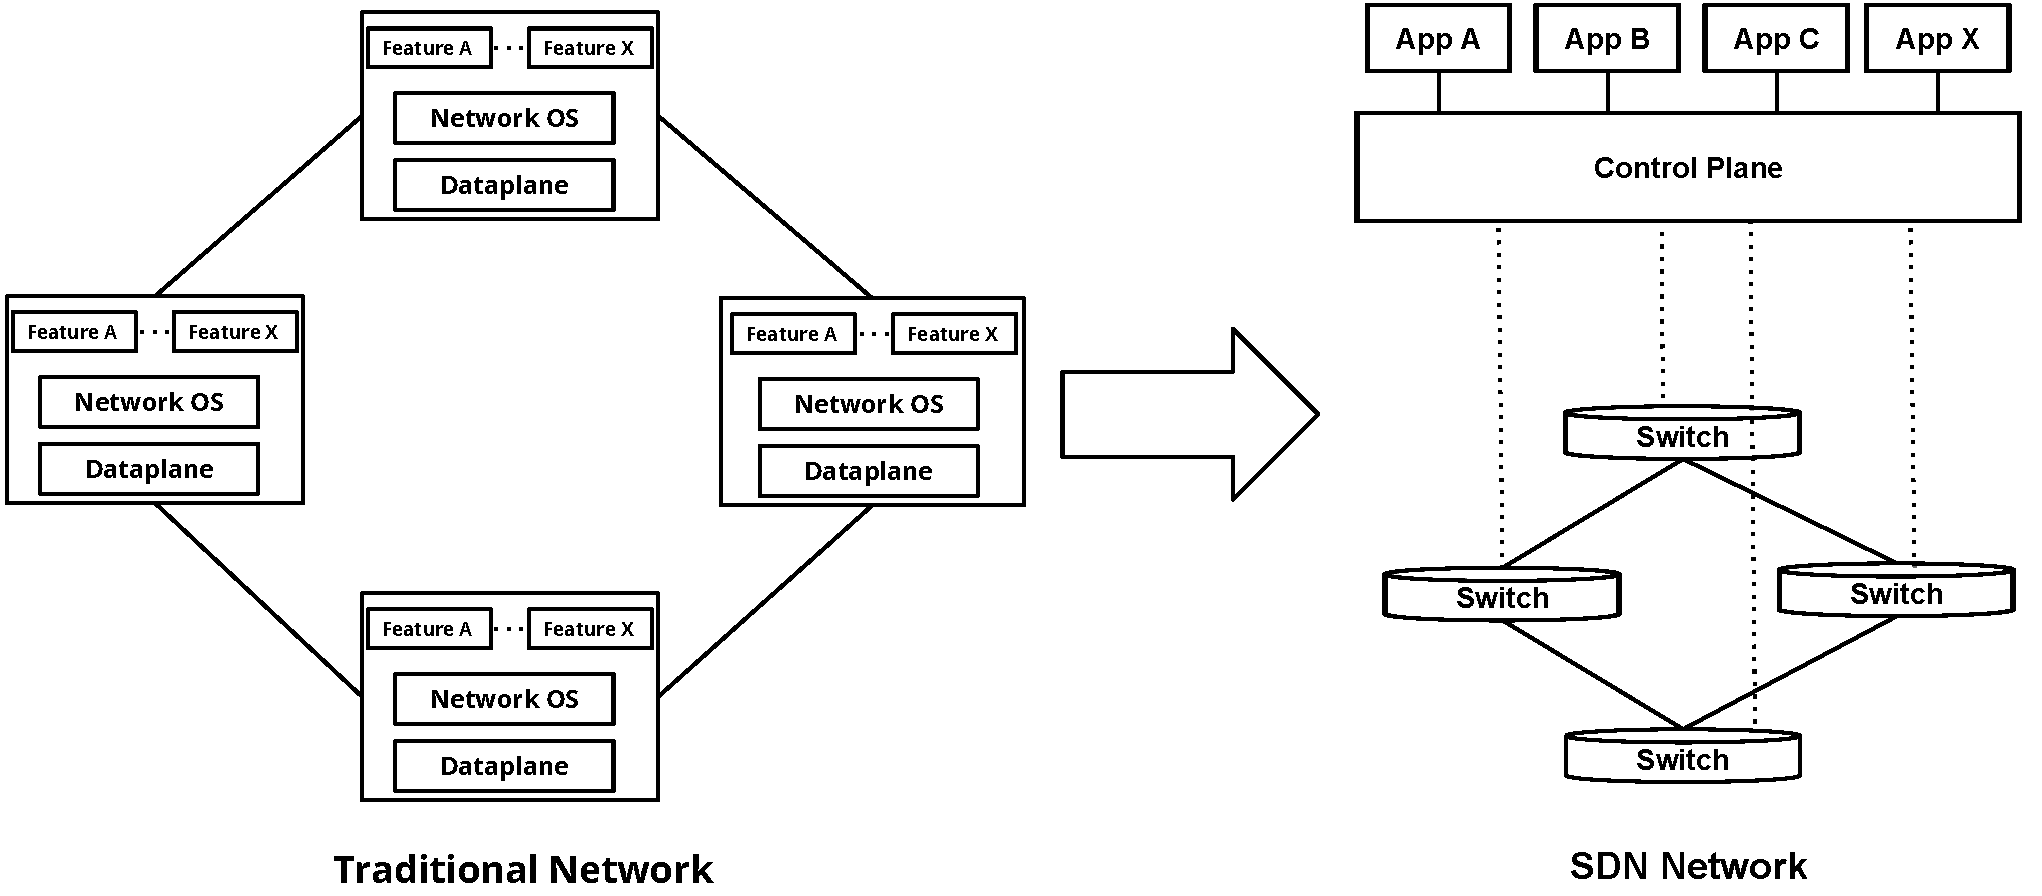
\includegraphics[width=\textwidth,keepaspectratio]{cap1/TraditionalvsSDN.pdf}
\caption{Traditional and SDN models}
\label{fig:traditional_vs_sdn}
\end{figure}
    
The first and the most common standard southbound interface for SDN is the OpenFlow protocol \cite{McKeown:2008:OEI:1355734.1355746} \cite{2012onf_sdn}. The OpenFlow specification describes the interaction between an OpenFlow compliant switch and an OpenFlow controller. Basically the controller installs flow entries for the   switch flow table, so the switches may apply instructions based on the network traffic.


\section{Motivation}
\label{sec:sec01}

Among the reasons for the fast evolution of the OpenFlow protocol is the experimental work led by researchers from Standford, where the protocol was born. New features and capabilities were validated on a software switch implementation, allowing researchers to create and to try new control plane applications. Soon, advances and emerging use cases took the industry attention for SDN and OpenFlow. This culminated in the creation of the Open Network Foundation (ONF), an organization composed by big network players and vendors, as by emerging startups. This organization became responsible for new OpenFlow versions since the version 1.2 and started working on new and enhanced features, resulting in the version 1.3 less than one year after 1.2. 

On the other hand, OpenFlow controllers and switches did not follow the protocol advancements, notwithstanding the fast evolution, resulting in lack of alternatives to experiment new capabilities and anticipation of new applications that could benefit from new features.

With this scenario in mind we found the emerging need to upgrade these tools, allowing fast experimentation and validation. By keeping up the pace with OpenFlow new versions, we expect to contribute to the future of the protocol, driving companies and researchers to develop applications in the state of the art and  enabling future OpenFlow version to be build and tested upon our work.  

\section{Objectives}
\label{sec:sec02}

The objective of this work is the development of a programmable OpenFlow 1.3 software switch to enable fast, real and flexible experimentation for SDN research and education on OpenFlow networks. To achieve this, the software switch must meet the following requirements:  

\begin{enumerate}

\item  \textbf{OpenFlow protocol feature completeness.} All required and optional features shall be implemented, allowing a full OpenFlow experience, without limitations for SDN researchers and developers.   

\item  \textbf{Code simple, easy to prototype and extend.} The code must be simple enough to be modified by anyone with a basic level of programming and understanding of OpenFlow. For this reason, easy insertion of features should be favored in lieu of performance. This requisite meets research needs that goes beyond the OpenFlow specification (e.g: the addition of new messages, new algorithms for group processing, changes to the pipeline, etc). Also, it encourages and helps users to search and to fix bugs quickly, preventing work interruption while waiting for an official patch to correct the switch.       

\item  \textbf{Straight forward integration with experimentation environments and emulation tools.} The switch must integrate with both real and emulated environments, ensuring seamless communication with other switches and controllers, without great modifications. Minor changes are acceptable due to specific platforms requirements: for instance, different processor architectures.

\item \textbf{Maximum throughput equal or higher than 100 Mbps.} High performance is not one of the project goals. However, there are features that play with the switch packet rate. Therefore, for a significant user experience, the switch must be able to support rates of at least 100 Mbps. This value was estimated based by the minimum bandwidth required by common Internet applications. Table \ref{tab:appband} is a mix from values obtained by \cite{Chen:2004:QRN:1234242.1234243} and some popular Internet services. Considering the applications and the bandwidth usage, we found that 100 Mbps is a value to perform a reasonable number of different experiments.          

\begin{savenotes}
    \begin{table}[h]
    \centering
    \caption{Minimum bandwidth requirements for common internet applications}
    \label{tab:appband}
    \begin{tabular}{|l|l|l|}
    \hline
    \textbf{Application}          & \textbf{Bandwidth (Mbps)}                         \\ \hline
    Web Browsing                      & 0.038                                        \\ \hline
    Email                             & 0.01                                          \\ \hline
    Telnet                            & < 0.001                                          \\ \hline
    Audio Broadcasting                & 0.08 to 0.375\footnote{Spotify - https://support.spotify.com/us/learn-more/faq/\#!/article/What-bitrate-does-Spotify-use-for-streaming}                                          \\ \hline
    Video Broadcasting                & 0.5 to 60 \footnote{Netflix - https://help.netflix.com/en/node/306}                                          \\ \hline
    
    \end{tabular}
    \end{table}
\end{savenotes}

\end{enumerate}

\pagebreak
\section{Text Structure}
\label{sec:sec03}

In this Introduction we explained the motivational aspects that justify this work. Also, we give a clear explanation for the objectives of this project. 

In Chapter~\ref{cap:cap02} we present a Literature Review. Related OpenFlow software switches' current functionalities are discussed from the point of view of our implementation requisites. Furthermore, we introduce other tools which are important parts of the OpenFlow ecosystem. 

In Chapter~\ref{cap:cap03} we take a look at the architecture of the software switch which is compliant with OpenFlow 1.3. We explain the modules relationship and roles within the OpenFlow pipeline.

In Chapter~\ref{cap:cap04} we highlight implementation details of OpenFlow 1.3 features in our architecture.  

In Chapter~\ref{cap:cap05} we evaluate the software switch in terms of common OpenFlow benchmarks and compare with related work.

Finally, in Chapter~\ref{cap:conclusion} we give our conclusion remarks. This chapter highlights results, presents known use cases and discusses possible improvements in future works. 
\chapter{Literature Review}
\label{cap:cap02}

OpenFlow is the central theme of this project and the OpenFlow 1.3 specification \cite{ofspec13} is the main document of our bibliographic base. For this reason, a deep study of the protocol and technologies that use it was carried out. We have evaluated and compared available implementations of other OpenFlow software switches. Also, some tools required evaluate our work are worth mentioning. We investigated controllers, test frameworks and packet dissectors, all candidates to compose our OpenFlow test environment. The next sections will give an overview about OpenFlow and relevant tools related to this work. 

\section{OpenFlow}
\label{sec:sec21}

OpenFlow is an open standard communication interface between switches and controllers, allowing centralized control and programmability in the network. The basic OpenFlow switch is composed by one or more flow tables, a group table and one or more OpenFlow channels for communication with OpenFlow controllers. Figure \ref{fig:logicalswitch} is a logical view of the minimal elements required by an OpenFlow switch. 

\begin{figure}[H]
\centering
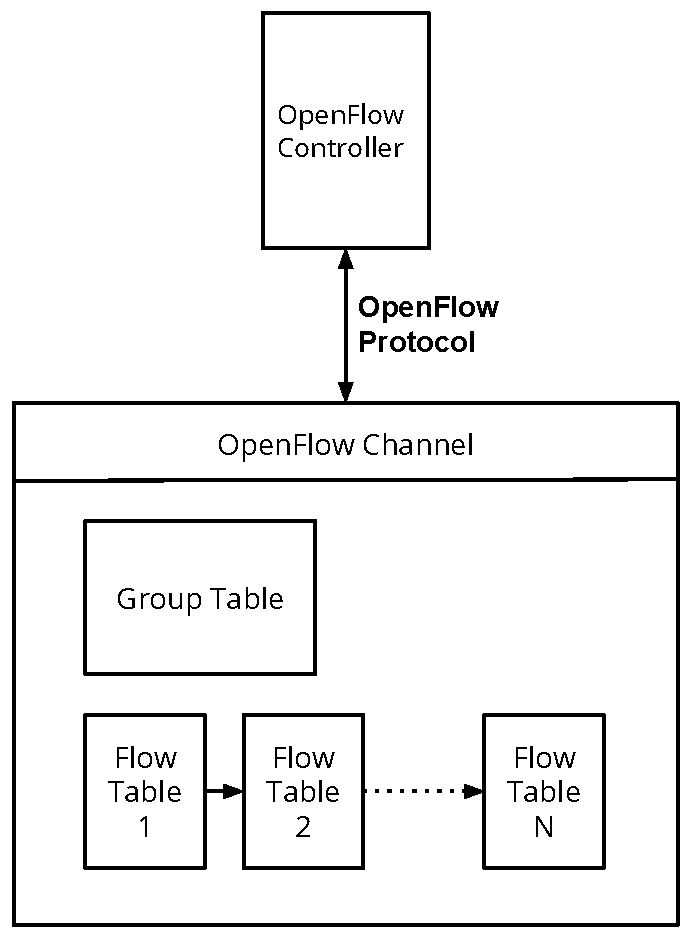
\includegraphics[height=8cm,width=\textwidth,keepaspectratio]{cap2/OFSwitch.pdf}
\caption{OpenFlow switch minimal elements.}
\label{fig:logicalswitch}
\end{figure}
\pagebreak

OpenFlow controllers can install flows into the switch flow table. A flow consists of match fields, counters and instructions applied to matching packets. A packet matches a flow if the protocol header field's values are the same as those specified in flow match fields. The most recent version requires 13 match fields, shown by Table \ref{tab:OFRequired}, but has optional support for more than 30 protocols fields from layers 2, 3 and 4 of TCP/IP network stack.

The OpenFlow pipeline starts at the first flow table and continues to additional tables. Flows are matched in order of priority and the associated instructions are executed. Only two instructions are required for OpenFlow switches: \textit{Write-Actions}, in which actions are executed at the end of the pipeline, and \textit{Goto-Table}, to jump to tables with an id greater than the table where the instruction is executed. Optional instructions are \textit{Meter}, to direct the packet to some meter for Quality of Service (QoS), \textit{Apply-Actions}, for immediate action application, \textit{Clear-Actions}, to clear all actions written by a \textit{Write-Actions} instruction, and \textit{Write-Metadata}, to write metadata information to be carried across the tables. 

\begin{table}[H]
\caption{OpenFlow required match fields}\label{tab:OFRequired}
\centering
\begin{tabular}{|l|l|}
\hline
\textbf{Field} & \textbf{Description}                \\ \hline
Inport         & Ingress Port                        \\ \hline
Eth Dst        & Ethernet destination address         \\ \hline
Eth Src        & Ethernet source address              \\ \hline
Eth Type       & Type of the packet, after VLAN tags \\ \hline
IP Proto       & IPv4 or IPv6 next protocol number   \\ \hline
IPv4 Src       & IPv4 source address                 \\ \hline
IPv4 Dst       & IPv4 destination address             \\ \hline
IPv6 Src       & IPv6 source address                 \\ \hline
IPv6 Dst       & IPv6 destination address            \\ \hline
TCP Src        & TCP source port                     \\ \hline
TCP Dst        & TCP destination port                \\ \hline
UDP Src        & UDP source port                     \\ \hline
UDP Dst        & UDP destination port                \\ \hline
\end{tabular}
\label{my-label}
\end{table}

Actions can perform modifications on packets, discard or send them to the group table or simply output to some specific port. The only required actions are \textit{Output}, to send the packet through a port, and \textit{Drop}. The packet modification actions are all optional, but their implementation is recommended, as they give more power and options to OpenFlow networks. The optional actions are \textit{Group}, to process the packet through a specific group; \textit{Push-Tag/Pop Tag}, for addition and deletion of VLAN, MPLS and PBB tags; \textit{Set-Field}, to modify packets header fields; \textit{Change TTL}, an action to modify MPLS and IP TLL; \textit{Set-Queue}, to determine which queue is attached to a port and will be used for scheduling in packet forwarding.

OpenFlow groups are a way to perform more complex forwarding actions. When a packet is sent to a group it is cloned and executed by sets of action buckets. This abstraction enables flooding, multipath, link aggregation and other techniques that demand transmission of packets through more than one port. 

The last essential block is the OpenFlow channel. The main connection between controller and switch is done by one of the following transport protocols: TCP or TLS, where the second is recommended because it enables data encryption of the transmitted data. Auxiliary connections are also allowed and it is possible to have UDP connections for transmission of less sensitive OpenFlow messages.

An optional element of the OpenFlow switch is the Meter Table. This table comprises different types of Meter Bands, which have a speed limit and apply a determined QoS action in the case of a packet flow exceeding the determined limit. There are two types of bands covered by the OpenFlow 1.3 specification: \textit{Drop}, to discard packets; and \textit{DSCP Remark}, to decrease the drop precedence of the DSCP field of the IP header.

\subsection{One day in the life of an OpenFlow 1.3 switch in 10 steps}

To illustrate the operation of an OpenFlow switch we will present a common and simple example for new SDN learners. A learning switch is a layer 2 network equipment that learns the port to which a host is connected. Learning happens when a packet from a host arrives at the switch for the first time. The switch then obtains and stores the host Media Access Control (MAC) address associated with the port number. Next time, when another host sends a packet to the previous learned address, the switch will forward it directly, instead of flooding to all ports. 

In legacy devices, the control software is embedded into the switch hardware and the MAC addresses are stored in a Content Addressable Memory (CAM) table. In an OpenFlow scenario, the learning happens inside the controller and the forwarding rules are stored in the Flow Table. We will describe the steps of learning and forwarding processes of an OpenFlow switch controlled by a simple learning switch application, considering the topology in Figure \ref{fig:simpletopo}. 

\begin{figure}[H]
\centering
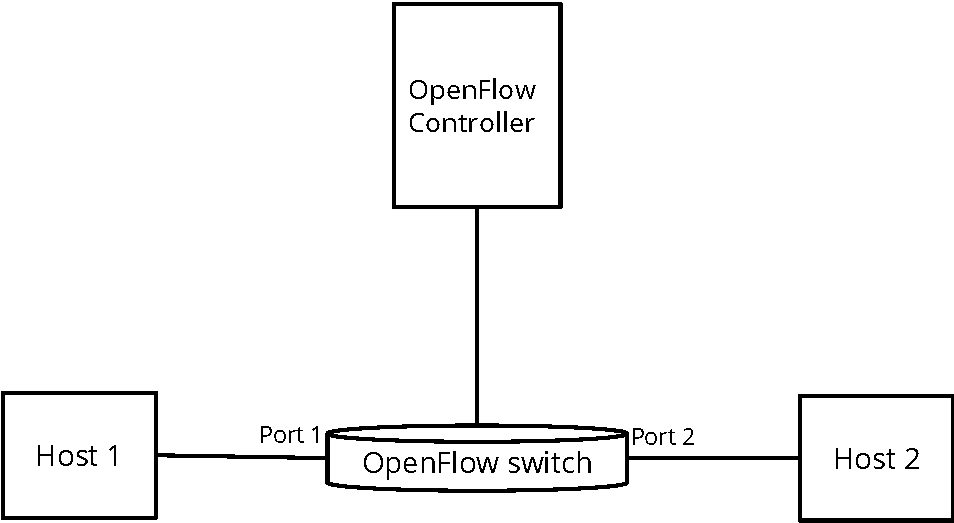
\includegraphics[height=5cm,width=\textwidth,keepaspectratio]{cap2/SimpleTopology.pdf}
\caption{Simple topology for the learning switch example.}
\label{fig:simpletopo}
\end{figure}

In the initial state the switch Flow Table is empty, \textit{Host 1} and \textit{Host 2} do not know anything about each other and the  \textit{Controller} is about to connect with the \textit{Switch}. 

\begin{enumerate}

\item The \textit{Controller} establishes a connection with the \textit{Switch}. As packets sent to an empty Flow Table are dropped according to the OpenFlow 1.3 specification, the  \textit{Controller} installs a low priority flow to direct every non matching packet to him. Table \ref{tab:initialtable} shows the Flow Table state after the installation of the first flow.  

\begin{table}[H]
\centering
\caption{Switch Flow Table state after controller connection}
\label{tab:initialtable}
\begin{tabular}{|l|l|l|}
\hline
\textbf{Match}  & \textbf{Priority} & \textbf{Instruction}                              \\ \hline
all             & 0                 & apply actions -> output:controller                \\ \hline
\end{tabular}
\end{table}

\item \textit{Host 1} wants to transmit a file to \textit{Host 2}. As it does not know about \textit{Host 2} MAC address, it sends an ARP \cite{rfc826} request to the network.

\item The ARP request packet enters the \textit{Switch} and matches the unique flow installed in the Flow Table. The action is applied, sending the packet to the  \textit{Controller} in an OpenFlow \textit{Packet In} message.

\item The  \textit{Controller} receives the \textit{Packet In}. The message contains information about the packet input port and headers. The  \textit{Controller} application learns and stores the \textit{Host 1} input port and MAC address. After that, it sends a \textit{Packet Out} message back to the \textit{Switch}, with an action to flood the packet in every \textit{Switch} port.   

\item The \textit{Packet Out} message arrives at the \textit{Switch} and the packet is flooded to every port, except the port where it came from.

\item The ARP request is delivered to \textit{Host 2}. Then, an ARP reply is sent back with the \textit{Host 2} MAC address required by \textit{Host 1}.

\item The ARP reply arrives at the \textit{Switch}. It matches the only present flow and is sent in a \textit{Packet In} message to the  \textit{Controller}.   

\item Now, the  \textit{Controller} checks if the packet MAC address is known. As the address is not present, it stores the input port and the MAC. Now it checks if the destination address was stored previously. The destination to \textit{Host 1} is already known. The  \textit{Controller} installs a new flow into the \textit{Switch} Flow Table. The flow illustrated in the second row of Table \ref{tab:secondtable} matches every packet destined to \textit{Host 1} MAC address and outputs the packet into port 1. After installing the flow, it sends the ARP reply to the \textit{Switch}, encapsulated in a \textit{Packet Out} message.

\begin{table}[H]
\centering
\caption{Switch Flow Table state after learning Host 1 address}
\label{tab:secondtable}
\begin{tabular}{|l|l|l|}
\hline
\textbf{Match}                 & \textbf{Priority}   & \textbf{Instruction}                              \\ \hline
all                            & 0                   & apply actions -> output:controller                \\ \hline
eth dst:HOST 1 MAC             & 100                 & apply actions -> output:1                         \\ \hline
\end{tabular}
\end{table}

\item This time The ARP reply is not flooded to all ports. As the  \textit{Controller} knew about the destination, it is sent directly to \textit{Host 1}. After receiving the ARP reply, it starts transmitting the file to \textit{Host 2}.

\item Again, the first packet of the file transference to \textit{Host 2} is sent to the  \textit{Controller}. Now it knows about \textit{Host 2} MAC and origin port. It installs another flow, shown in the third row of Table \ref{tab:finaltable}, and it sends the \textit{Packet Out} message to the \textit{Switch}. The \textit{Switch} sends the packet directly to \textit{Host 2}. From now on, the packets are not sent for the \textit{Controller} anymore because the installed flows are matched. 

\begin{table}[H]
\centering
\caption{Switch Flow Table final state}
\label{tab:finaltable}
\begin{tabular}{|l|l|l|}
\hline
\textbf{Match}                 & \textbf{Priority}   & \textbf{Instruction}                              \\ \hline
all                            & 0                   & apply actions -> output:controller                \\ \hline
eth dst:HOST 1 MAC             & 100                 & apply actions -> output:1                         \\ \hline
eth dst:HOST 2 MAC             & 100                 & apply actions -> output:2                         \\ \hline
\end{tabular}
\end{table}


\end{enumerate}        

\section{OpenFlow software switches}
\label{sec:sec22}

OpenFlow software switches play an important role in the protocol evolution. At first, they were a low cost solution to create and experiment your own SDN applications in a controlled and smaller environment, before the deployment in a production environment. With the new SDN approaches for network virtualization \cite{Tseng:2011:NVC:2117686.2118540} \cite{Drutskoy_scalablenetwork}, software switches have been receiving a lot of attention from the industry \cite{NSX} and academy \cite{DBLP:confcloudnetEmmerichRWC14}. SDN virtual switches interconnect virtual machines from data center tenants and help scaling a plethora of traffic engineering applications. For instance, tenant isolation is easily achieved using an OpenFlow software switch to connect virtual machines. Usually, it is implemented using VLAN segregation, which is not scalable for more than 4096 tenants (the total number of possible VLAN identifiers). In turn, OpenFlow switches offer more granular options to segregate the network hosts, due to the number of fields available for flow matching, which eliminates the need to segregate hosts only in a layer 2 domain.

\begin{table}[H]
\caption{Comparison of OpenFlow software switches}
\label{tab:relatedswitches}
\begin{tabular}{|l|l|l|l|l|}
\hline
\textbf{Switch} & \textbf{Language} & \textbf{Emulation tool integration} & \textbf{Mode}    & \textbf{OF-Config} \\ \hline
Reference       & C                 & Yes                        & userspace        & No                         \\ \hline
Open vSwitch    & C                 & Yes                        & userspace/kernel & No                         \\ \hline
LINC            & Erlang            & No                    & userspace        & Yes                        \\ \hline
Trema           & C/Ruby            & No                    & userspace        & No                         \\ \hline
\end{tabular}
\end{table}

Before the implementation, we investigated four OpenFlow software switches that supported OpenFlow 1.0, since there was no sense in implementing basic OpenFlow features from scratch. Table \ref{tab:relatedswitches} is a comparison of the examined software switches and reflects their state in the year of 2012. The columns are related to the objectives defined in chapter \ref{cap:intro}. Language is an important element, since popular programming languages have the power to reach bigger audiences. The integration with emulation tools eases experimentation and speeds up testing. The mode column is related to switch performance, since a kernel space implementation tend to be more efficient than an user space implementation. In a kernel implementation, packets are processed directly in the kernel space, eliminating the overhead of traversing packets between the kernel and user space.

In the mean time of this work, most of the analysed software switch projects started to add support for newer OpenFlow versions. Figure \ref{fig:ofswitchtimeline} shows the switche's timeline for the implementation of most recent OpenFlow versions. Colored intervals show that these OpenFlow versions are still in progress or do not include all features described on the specification, as will be shown in section \ref{sec:FeatureComplete}.

\begin{figure}[H]
\centering
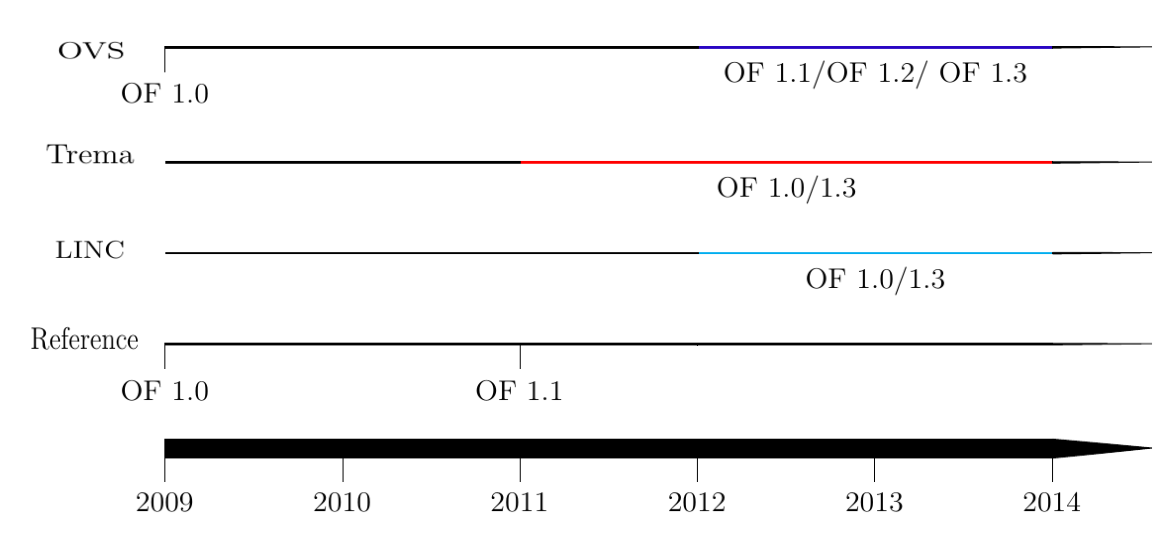
\includegraphics[height=6cm,width=\textwidth,keepaspectratio]{cap2/SoftSwitchTimeline.pdf}
\caption{OpenFlow Software Switches: version support timeline.}
\label{fig:ofswitchtimeline}
\end{figure}

The next subsections will provide a short individual description of the software switches investigated: OpenFlow reference switch, Open vSwitch, LINC and Trema. 

    \subsection{OpenFlow reference switch}
    \label{sec:sec221}
    
     The first OpenFlow switch is known as reference switch because it was implemented by Stanford researchers directly involved with the OpenFlow protocol creation and the first specification releases. The code is written using the C language and its simplicity is one of the reasons for the implementation to other platforms. Two important ports are: NetFPGA boards \cite{netpfgaof}, eliminating the disadvantage of the user space implementation; and OpenWrt \cite{pantou} for wireless routers. These efforts enabled low cost options to test OpenFlow on real hardware during earlier protocol stages.    
     
     The last OpenFlow version implemented by Stanford researchers was 1.0, but after the version 1.1 release there was an update, based on the reference switch, released by Ericsson Traffic Lab, called of11softswitch \cite{of11softswitch}. To conform changes such as multiple tables, the switch forwarding plane was rewritten, but still retained all of the base software switch characteristics.     

     \subsection{Open vSwitch}
    
    Considered the \texttt{de facto} switch for virtual networks, Open vSwitch \cite{Pfaff_e.a.:extending} (OVS) is a mature and constantly evolving open source project. The efficiency provided by the kernel module and the functionalities beyond OpenFlow turns OVS into a great solution to replace the original Linux bridge. Although high performance is guaranteed by the kernel module, it makes the OVS code harder to insert new functionalities. 
    
    In addition to the basic connectivity provided by traditional bridges, OVS offers a flexible option to manage and program the packet forwarding behavior. OVS uses another protocol than OpenFlow for switch management. The Open vSwitch Database Management Protocol (OVSDB) is one of the most praised OVS features and is designed to manage all running switch instances, permitting the control of distributed virtual network nodes. With OVSDB, a network engineer can create, configure and delete OVS ports and tunnels from a centralized location.

    \subsection{LINC}
    
    LINC \cite{linc} is an userspace software switch written in the Erlang programming language and has different support levels, considering the number of working features, for OpenFlow versions from 1.2 to 1.4. The main advantage of this switch is the support to OF-CONFIG \cite{ofconfig}, the OpenFlow switch configuration protocol. As an userspace implementation, efficiency is not one of its strong points. However, it promises flexibility, fast development and testing of new OpenFlow features. 
    The Erlang language is not a disadvantage \textit{per se}, but it can be considered a blocking point for developers who want to add their own features. Erlang developers are growing, but their number are still very far from languages like C and Java.

    \subsection{Trema}
    
    Trema is a name known by the OpenFlow community for being a controller implementation project. However it goes beyond,  offering a full OpenFlow framework with the tools needed to develop OpenFlow applications \cite{trema}, including an OpenFlow software switch. Also, the framework has its own emulation tool for OpenFlow networks and end-hosts. The main repository of this project features switch with only OpenFlow 1.0. However, there is a repository known as trema-edge where the work for OpenFlow 1.3 is on progress.

\section{OpenFlow Controllers}

    Controllers are considered the brain of an OpenFlow network. Every configuration and forwarding rules are defined by applications running on top of a controller. They are sent in form of OpenFlow messages, which have to conform with the format defined by the specification. For this reason, we need to validate our work testing interoperability between the software switch and a compliant controller. We reviewed the main open source projects, looking for an OpenFlow 1.3 controller or an easy alternative to implement some level of support for OpenFlow 1.3, required for our tests. 

    \subsection{NOX}

    One of the first open source OpenFlow controllers, NOX \cite{nox} was very famous during the first years of OpenFlow. Its popularity was due to a combination of factors, from the C++ implementation and a Python binding, which helped to speed up the prototyping, to a quite simple interface and a good number of example applications. The last official release supported OpenFlow 1.0 version. After some enhancements on the controller speed \cite{nox-mt}, no efforts were made to upgrade it for newer OpenFlow versions. 
    
    \subsection{POX}
    
    Pox is a controller implemented in Python and can be considered a NOX sibling \cite{pox}, created to address the lack of speed when prototyping with NOX. Its main goal is to become the archetypal of a modern SDN controller, featuring some desired SDN capabilities like debugging, new programming models and network virtualization. 
    
    Designed with research in mind, under constant development and a typical controller used for SDN education, POX was a great candidate to be the controller for testing the software switch, but the OpenFlow support still doesn't surpass version 1.0
  
    \subsection{Floodlight}

    The Floodlight controller is a popular OpenFlow controller backed by Big Switch Networks, one of the most prominent SDN startups \cite{floodlight}. It is developed in Java and was designed for high performance and is the core of Big Switch Networks' commercial solution. One of the greatest features of Floodlight is the module loading system that makes it very extensible, allowing it to enable and disable applications at run time. Another great feature is the Open Stack integration, a cloud orchestration platform. Floodlight instances control the virtual switches linking virtual machines orchestrated by Open Stack. Regarding OpenFlow version support, it currently supports OpenFlow 1.0 and 1.3. 
  
    \subsection{Ryu}
    
    Ryu is considered an SDN network framework \cite{ryu}, an abstraction that provides code software components, with generic functionality, easing and speeding development of SDN applications. It is implemented in Python, like POX, but has a different architecture. Designed as software components, developers can create OpenFlow applications like modules. Furthermore, the controller also supports management protocols like OF-Config and Netconf.
    
    Very well documented, with a large number of examples and featuring all OpenFlow versions, Ryu is currently a great choice to test the software switch, but when we started this work OpenFlow support was limited to OpenFlow 1.0. OpenFlow 1.3 support was only available in the middle of our switch implementation.
 

\section{OpenFlow test and emulation}
\label{sec:testemulation}
    The last pieces of a minimal OpenFlow environment are  test frameworks and emulation tools. For our development we are more interested in the first, though a modular emulation software compatible with our software switch may benefit users looking for a complete, controlled and easy to setup testbed. 
    
    \subsection{OF-Test}
    
    OF-Test was the first OpenFlow test framework. Developed by the same team working on Floodlight, OF-Test \cite{oftest} tests basic functionality for OpenFlow 1.0 and 1.1, with 1.2 and 1.3 currently in development. The simpler architecture and Python implementation turns it into a very easy and fast platform to create and run tests. It works connecting the OF-test server to the switch control and the data plane. The server is responsible for monitoring OpenFlow messages and packets sent through and along the planes. If these messages and packets are according to expected results, the test returns OK, otherwise, a failure is reported.
    
    \subsection{Ryu Test Framework}
    
    This test framework is part of the Ryu controller and implements tests to cover all, required and optional, OpenFlow 1.3 and 1.4, actions, instructions and match fields, with a more comprehensive test than OF-Test. The test cases are written in JSON, so there is no need for coding to create a test, which enhances the speed of test creation. 
    
    There is an online certification which continuously tests OpenFlow software and hardware switches, including our work \cite{ryucert}. Results from this certification will be presented in chapter \ref{cap:cap05}.

    \subsection{OpenFlow packet dissectors}

    Packet dissectors are important tools to test if message packets are correct or to check if an specific packet was sent or modified by an OpenFlow output and set-field actions, respectively. Wireshark \cite{wireof} is the most famous program to dissect packets. Although a wide range of protocols are officially supported, OpenFlow support started as an  unofficial  plugin for OpenFlow 1.0 and 1.1. For a long time this plugin was the only option for analyzing OpenFlow traffic. Recently, due to the growth in the number of users requesting for official support, OpenFlow is now developed in the dissector's main repository \cite{wireof}.    
    \subsection{Mininet}
    
   Mininet \cite{Lantz:2010:NLR:1868447.1868466} is a tool for network emulation. In a single machine it runs switches, links and hosts just like a complete virtual network. It is possible to log into the hosts and use programs like Iperf \cite{iperf} and Ping, to measure throughput and check connectivity; specify link parameters as speed and delay; and instantiate a network topology composed of software switches. The capacity to create and to destroy virtual networks allows fast and easy experimentation. 
  
    
\chapter{Architecture}
\label{cap:cap03}

Architectural design is strongly tied down by OpenFlow 1.3 required and optional elements. With the architecture description, we do not intend to repeat the specification. Thus, elements described in the next sections are an specific and conceptual point of view of each software switch component. 

The OpenFlow switch implementation is a fork from the OpenFlow 1.1 reference switch. We choose this implementation as a starting point for our work because of the simpler code base, when compared to other switch implementations discussed in section \ref{cap:cap02}. Although simple, the only documentation available to understand the reference switch was the OpenFlow specification. For this reason, the definition of the architectural design started from the extraction of the previous software architecture. 

Firstly, through a simple reverse software engineering process \cite{Sommerville:2001:SE:375369}, we analyzed the code and listed the switch core components. Next, we identified missing components from the OpenFlow 1.3 specification. After these steps, we found that block structures suggest the application of a bottom-up design \cite{vonMayrhauser:1990:SEM:79005}. In this approach, the basic set of foundational modules and their interrelationships are the foundation for the final architecture. Following these concepts, we came up with the final design for the OpenFlow 1.3 software switch.

In the Figure \ref{fig:switcharq} we show the software switch architecture. The most important block is the Datapath. It consists of OpenFlow internal elements such as Flow, Meter and Group Tables, and a Packet Parser as well. The other three blocks operate on different levels along with the Datapath. From the top level, the blocks Datapath, Marshaling/Unmarshaling library and Communication Channel are part of the OpenFlow message layer. Below, Ports and Datapath form the network packets layer, where packets arrive, are processed and usually sent back for the network.\footnote{Some instructions, actions and even an empty table may cause a packet drop in the Datapath.} Except for the special case of the \textit{Packet In} message, in which packets can be sent for the controller, these two layers do not interact. In Figure \ref{fig:switcharq}, dotted lines illustrate some possible paths a network packet can travel between the Ports and the Datapath. Solid lines denote the OpenFlow messages traveling in the OpenFlow message layer. Arrows mean the direction packets and OpenFlow messages can take across the switch components. In this chapter, we present each software switch component individually, detailing each block roles and interactions with other elements.

\begin{figure}[H]
\centering
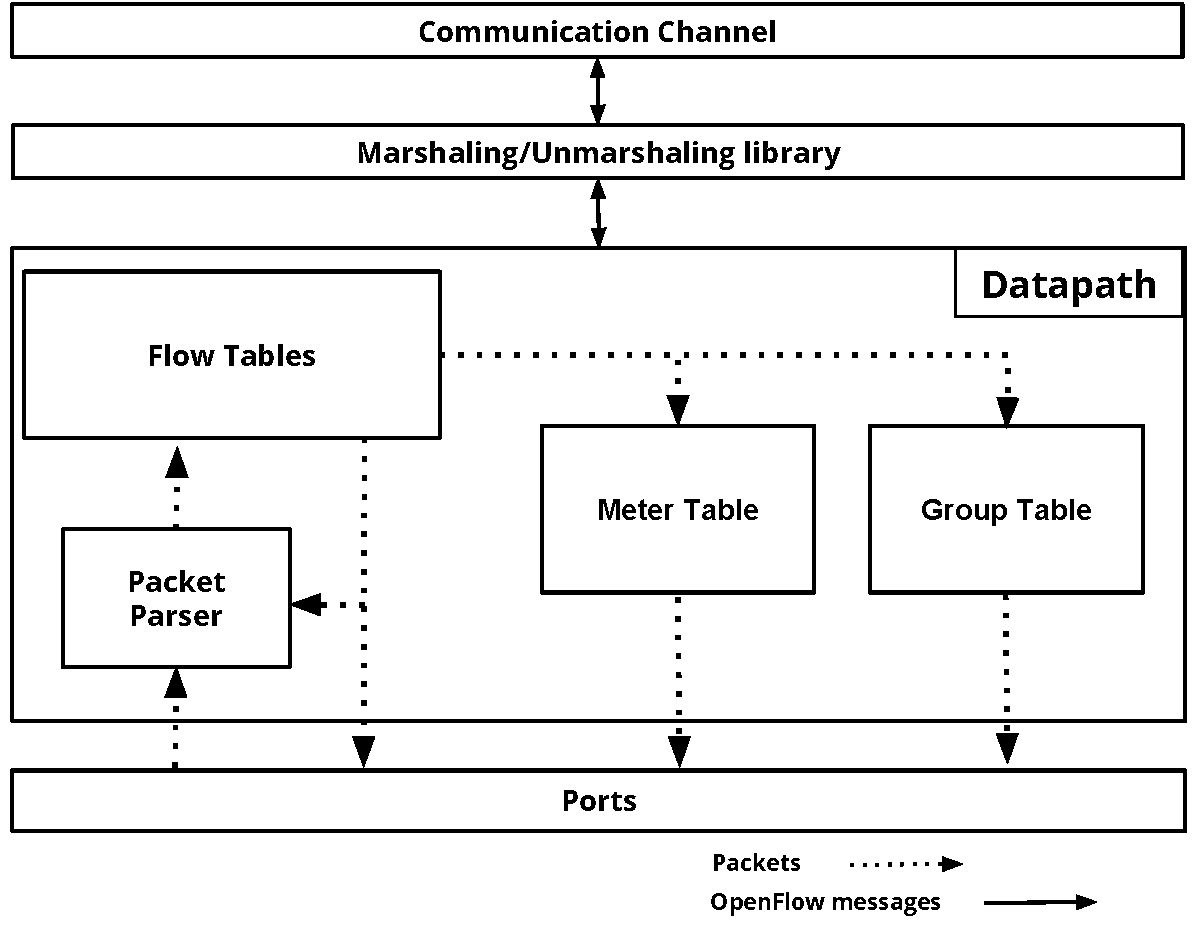
\includegraphics[height=12cm,width=\textwidth,keepaspectratio]{cap3/switcharq.pdf}
\caption{Software switch architecture}
\label{fig:switcharq}
\end{figure}

	\section{Ports}

	OpenFlow ports are the entrance and exit doors for  network packets of the OpenFlow switch pipeline. A software switch instance running on a machine may use their physical or virtual interfaces as port elements. Physical port elements can take control over Ethernet or WiFi interfaces, allowing the creation of real network topologies. Although limited by the speed of the software switch, the possibility to create a low cost testbed enriches the experience of users developing and testing OpenFlow applications.     

	Ports functions on the switch are not limited to the task of send and receive packets. There is a set of responsibilities associated with the OpenFlow protocol and the pipeline. Functionalities are:

	\begin{itemize}

	\item OpenFlow enables some level of control over a port behavior. A port modification message permits the configuration of the port state. Ports can be administratively set to drop all received or forwarded packets, forbid the generation of \textit{Packet In} messages from arriving packets, and brought down. Ports elements should handle these messages and change the port behavior according to the configuration sent.

	\item OpenFlow Ports keep the current state of the physical link. This information is not configurable by an OpenFlow controller, but the switch should inform the control plane about link state changes. Ports monitor the state of the port link and update the information according to changes.

	\item Packets encapsulated in \textit{Packet In} usually have only the header sent within the message. A buffer stores the packet, while waiting for the controller decision after the \textit{Packet In}. Ports elements store these packets and resend them for further processing.

	\item An OpenFlow controller can ask the switch about a port description. The software switch element retrieves information such as current and max operating speeds from the interfaces of the machine and stores it. On a port description request, the element handles the message and sends the required information to the control plane.

	\item Queues creation are not part of the OpenFlow protocol. However, OpenFlow can configure port queues, created by whichever mechanism, to be associated with a switch port. Ports are responsible for handling queue association and configuration.  

	\item Ports must update port and queue packet counters.           
	\end{itemize}

	\section{Packet Parser}

	Before entering the software switch OpenFlow pipeline, packet protocol fields are extracted by the Packet Parser element. Parsing packets was a formally defined task until OpenFlow 1.1. The main reason to define how packets should be parsed is to guarantee parsing consistency, but it limits switch designers and demands algorithm updates for each new protocol addition. For this reason, further specifications removed how packets should be parsed and match fields are now defined only logically.

	A Packet Parser element converts extracted protocol fields of a packet to an internal flow entry format. Two scenarios may trigger this function:   

	\begin{itemize}

	\item A network packet enters the switch through one of its ports.    

	\item  If the packet was modified by an action and is resubmitted for the pipeline, or sent to a table ahead by a \textit{Go To Table} instruction, packet revalidation is required. Hence the packet is processed by the Packet Parser again. In Figure \ref{fig:switcharq}, after passing by the Flow Tables, there is an arrow representing packet return to the Packet Parser.        

	\end{itemize}

	Further OpenFlow extensions, supporting new protocols, directly affect the packet parsing. Modifications are required in order to add new match fields for the Packet Parser. Therefore, a flexible and extensible Packet Parser element is desirable.  

	\section{Flow Tables}

	Flow Tables are the heart of an OpenFlow switch architecture. They are the elements where flow entries are stored and the OpenFlow pipeline starts. Although the use of multiple flow tables is optional - the specification mandates at least one table - its implementation is recommended, as even simple applications can not scale in switches with only one Flow Table \cite{tableExplosion}.  
	
	Flow Tables roles in the software switch are listed below.

	\begin{itemize}

    \item In case of nonexistence of a table miss flow entry, Flow Tables have to implement some default action for not matched packets. Currently, the default action is drop the packets. 

	\item Handle \textit{Flow Mod} messages sent by the controller. These messages may add or delete flow entries, or change the instruction set from currently installed flows.  

	\item Flow Tables must be able to have their capabilities reconfigured by a controller. These table features can express the table supported properties. The instructions' type and the match fields allowed in the table are examples of properties. Also, some fields show relevant information for an OpenFlow application. For instance, the table identifier value is an information required to add a new flow, and the max number of flow entries should be considered to avoid scalability problems.           

    \item A Packet look up must be performed upon the receiving of a packet. The operation looks for a flow table entry that matches the packet. In the case of a match, the switch executes the instruction set associated with the flow entry. This is the most common activity in Flow Tables.   
    
    \item Keep table statistics about the number of active flow entries, number of look ups and matched packets.  

	\end{itemize}

	\section{Group Table}

	Group Table empowers OpenFlow forwarding options. Packets reach the Group Table after matching a flow entry containing a group action, in one of the Flow Tables. 
	
	Group entries are stored into the Group Table. Each group entry contains an identifier, a type, counters and action buckets. Action buckets are an ordered list of action sets to be executed according to the group type. Figure \ref{fig:grouptable} represents a group table filled with groups of All, Indirect and Fast Failover types. The layout of the specific group types is important, because it defines Group Table attributions, as shown by the responsibilities listed here.
	
	\begin{figure}[H]
    \centering
    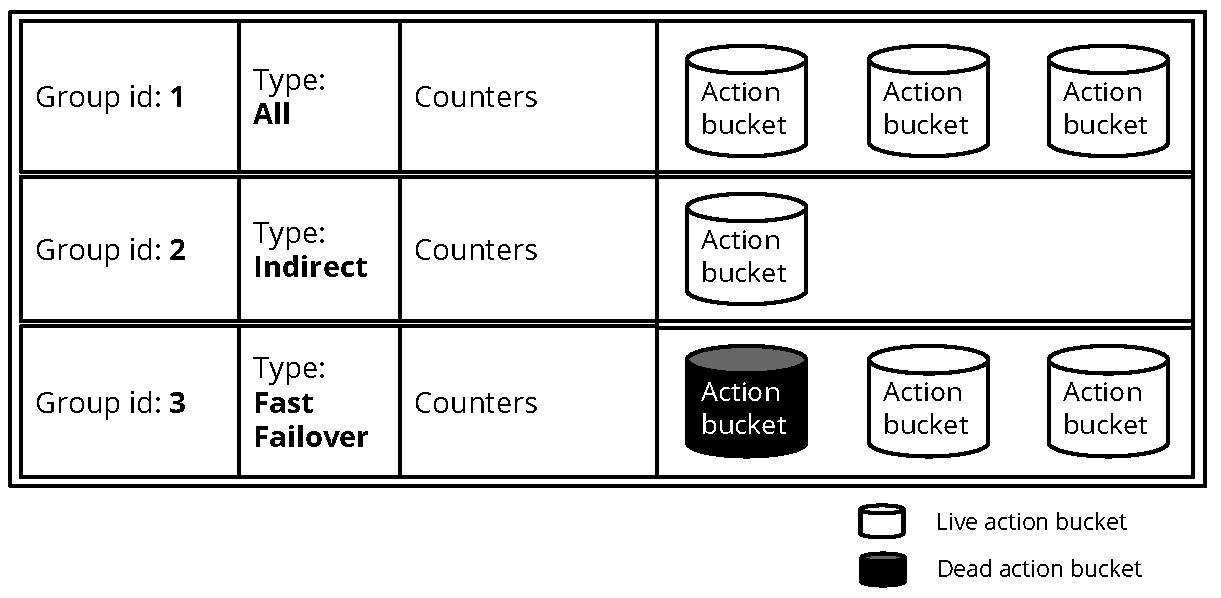
\includegraphics[height=7cm,width=\textwidth,keepaspectratio]{cap3/GroupTable.pdf}
    \caption{Group Table internals}
    \label{fig:grouptable}
    \end{figure}

	\begin{itemize}
	
	\item The Group Table have to guarantee group type restrictions. For instance, indirect groups support only one action bucket. 

	\item The Group Table must handle modification messages and perform consistency checks in the case of group chaining. Chained groups point to other groups and may cause loops that should be avoided by the element.  

	\item Fast failover groups require monitoring switch ports and group buckets for state changes. For this reason the Group Table is responsible for checking bucket liveness when choosing the first live bucket.

	\item A Group Table that supports the select group type has to implement a schedule discipline algorithm to choose which bucket will be applied to the packet.

	\end{itemize}

	\section{Meter Table}
	\label{sec:MeterTable}

    The Meter Table is an element to perform simple QoS operations. Per-flow meters are attached to flow entries through the \textit{Meter} instruction. A meter entry is composed by a meter id, counters and meter bands. The QoS operations to apply are defined by the meter bands. A meter band must have a type and rate value, which is the boundary to apply the action determined by the type. Figure \ref{fig:metertable} illustrates the internals of a Meter Table, with two meter band types.   

    \begin{figure}[H]
    \centering
    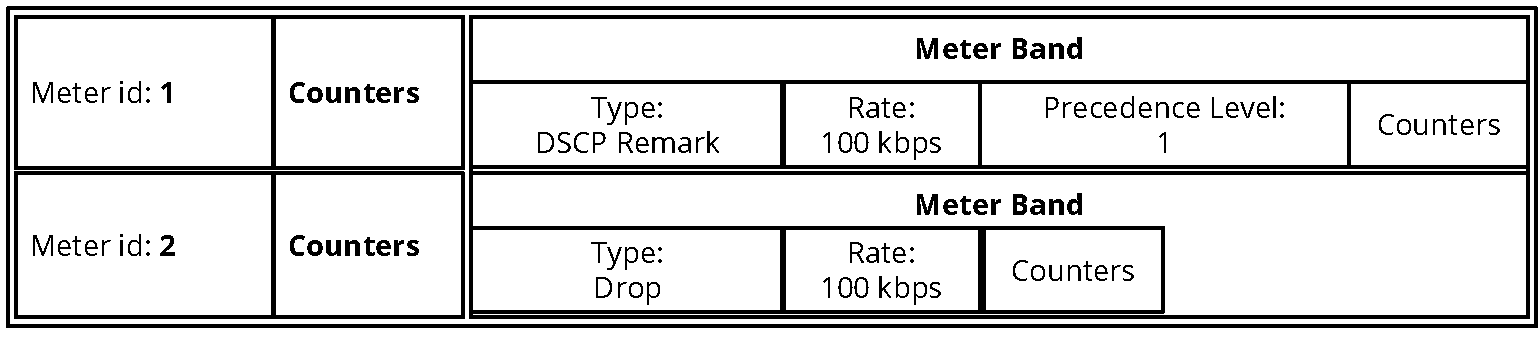
\includegraphics[height=7cm,width=\textwidth,keepaspectratio]{cap3/MeterTable.pdf}
    \caption{Meter Table internals}
    \label{fig:metertable}
    \end{figure}

    Meter Table responsibilities include:

    \begin{itemize}
    
    \item Creation, destruction and modification of meter entries.
    
    \item Matched packets, from flows pointing to the Meter Table, rate measurement. 
    
    \item Keep and update counters for statistics of packets processed by an entry.
    
    \item Process the packets according to band operation. A Drop meter band type discards the packets and the DSCP remark changes the IP packet drop precedence. 
    
    \end{itemize}

    \section{Marshaling/Unmarshaling library}
    \label{(un)pack}
    OpenFlow messages defined by the specification follow a proper format for transmission in the network. Messages are 8-byte aligned, so there may be insertion of padding fields to follow this alignment rule. Another requirement for the message format is the byte order. The preferred format for packets sent through the network is the network byte order \cite{rfc1700}. As OpenFlow messages are sent over IP networks, their messages should be assembled following the Big-Endian format.
    
    The architectures of machine's processor may operate on different byte-endianness. For instance, Intel processors use the Little-Endian byte order \cite{little-endian}. So, in order to handle and assemble OpenFlow messages, conversion is required for non Big-Endian architectures.     
    
    For the mentioned reasons, a library which abstracts byte-endianness and adds any required bytes to ensure right message format is required. A Marshaling/Unmarshaling library is not an element defined by OpenFlow specification. Its main function is the translation of OpenFlow messages from the network format to an internal format and vice-versa. The library responsibilities are the following:
    
    \begin{itemize}
    
    \item Every OpenFlow message must have a function that packs and unpacks it. Pack is the function which converts internal structures into network format. While unpack turns received messages into an internal structure.
    
        \subitem - When packing, the library has to add any necessary padding bytes.
        \subitem - On packing, the message should be assembled in network byte-order.
        \subitem - On unpacking, the library must translate the message fields to the switch host architecture byte-order.
    
    \item Some handling of OpenFlow message errors is done in this level. The library must raise errors for messages with wrong length or bad arguments. 
    
    \end{itemize}

    \section{Communication Channel}	

    The OpenFlow software switch communicates with controllers through the Communication Channel. This element connects with the Datapath and the controller and acts as a proxy between them. This element exists because the implementation of the communication channel is not defined by the specification. Since the message format is respected, implementations are free to choose the connection protocol. For instance, when security for the channel is a requirement, a protocol like TLS should be used to encrypt the messages. 
    
    In the software switch, the Communication Channel roles are:
    
    \begin{itemize}
    
    \item The Communication Channel must establish a TCP connection with the switch and the controller.
    
    \item Connection setup is a Communication Channel responsibility. After a TCP connection, the switch negotiates the protocol version with the controller. This process, known as handshake, is managed by the Communication Channel. 
    
    \item The channel may use multiple connections with a single controller at the same time. These connections can be used to send OpenFlow in parallel or to create specific channels for some message types.
    
    \item A Communication Channel is responsible for opening connections to enable switch communication with more than one OpenFlow controller. 
    
    \end{itemize}
    
    
    
\chapter{Development}
\label{cap:cap04}

This chapter covers the software switch development. In section \ref{softfeatures}, we give details about the implementation of the most important OpenFlow 1.3 features, in section \ref{OpenSourceDev}, we describe the open source model adopted for the software switch development. 

\section{Software switch implementation}
\label{softfeatures}

Implementation of an OpenFlow switch depends on the platform for which it is designed. OpenFlow hardware implementation on traditional Application Specific Integrated Circuit (ASIC) chips, usually suffer from limitations, like small capacity in the total number of flows and not real support for multiple tables. Unlike hardware, software implementations offer greater flexibility in the implementation of OpenFlow features. In environments where high throughput is not the biggest concern, software switches running on commodity servers can be a low cost replacement option for traditional network switches.

The OpenFlow specification describes OpenFlow switches pipeline and the required and optional building blocks. It does not gives low level details about how these components should be implemented. As long as it works how the specification dictates, switch designers are free to use any data structures and algorithms in order to implement OpenFlow. When defining implementation details, we explored the software implementation freedom to meet the requisites defined on section \ref{sec:sec02}. At the same time, we came up with innovative design decisions towards future extensions of the OpenFlow match field support.  

In this section we discuss how we implemented the OpenFlow 1.3 software switch adding several changes to the base switch - using C \footnote{In this chapter there will be two common words: struct and structure. While struct is a C language keyword and structure is a more generic word for a collection of data variables, both will be used to denote a C struct}, the switch native programming language, and C++ - in order to support all features and keep it as simple as possible. The next subsections describe this new functionalities in the context of the architecture of the software switch presented in chapter \ref{cap:cap03}.

\subsection{Oflib}
\label{sec:sec41}

The software switch architecture Marshaling/Unmarshaling library, presented in section \ref{(un)pack}, is called Oflib. Although already present in the software switch base code, the library underwent several modifications in old messages and grew with the addition of OpenFlow 1.3 messages.

Every OpenFlow message represented by the Oflib has a common header. This header struct contains only one member, which is the message type information. Using the same initial struct for every message struct allows the implementation of two general functions that abstract marshaling and unmarshaling. In the Listing \ref{msgpackunpack}, we show the definition of these functions. Marshaling, also known as packing, is done by \textit{ofl_msg_pack}. By passing a pointer to the struct \textit{ofl_msg_header} for the function, we can check the message type and apply the message respective marshaling function. Unmarshaling, also known as unpacking, is performed by \textit{ofl_msg_unpack}. In this function, the first bytes of the Openflow messages, the \textit{buf} parameter, reveal their types. With this information the function calls the proper function to convert the message for the Oflib format.  
\begin{lstlisting}[caption={Oflib: message pack and unpack base functions}, label=msgpackunpack,]
int ofl_msg_pack(struct ofl_msg_header *msg, uint32_t xid, uint8_t **buf, size_t *buf_len, struct ofl_exp *exp);

ofl_err ofl_msg_unpack(uint8_t *buf, size_t buf_len, struct ofl_msg_header **msg, uint32_t *xid, struct ofl_exp *exp);
\end{lstlisting}

Another Oflib task, discussed in the section \ref{(un)pack}, is message error handling. Checks for bad requests from the controller, like messages with unknown type and wrong size are performed by every unpacking function. In case of error, the function returns the OpenFlow error code for the Datapath, which creates an error message and sends it for the controller, through the Communication Channel.

Addition of new OpenFlow messages in the Oflib is a trivial task. Firstly, the developer needs to define a C struct, with \textit{struct ofl_msg_header} as the first member. Then, write a pack and unpack function. Finally, add the new message type for \textit{ofl_msg_pack} and \textit{ofl_msg_unpack}. Listing \ref{rolerequest} illustrates the OpenFlow 1.3 \textit{Role Request}, implemented during our work. 
\pagebreak
\begin{lstlisting}[caption={Oflib message Role request struct and function definition}, label=rolerequest,]
struct ofl_msg_role_request {
	struct ofl_msg_header header; /* Type OFPT_ROLE_REQUEST/OFPT_ROLE_REPLY. */
	uint32_t role;                /* One of OFPCR_ROLE_*. */
	uint64_t generation_id;       /* Master Election Generation Id */
};

static ofl_err
ofl_msg_unpack_role_request(struct ofp_header *src, size_t *len, struct ofl_msg_header **msg)

static int
ofl_msg_pack_role_request(struct ofl_msg_role_request *msg, uint8_t **buf, size_t *buf_len)
};
\end{lstlisting}

Additionally, the Oflib also has printing functions. This is helpful for logging and debugging in the software switch.      

\subsection{OpenFlow Extended Match}
\label{sec:sec42}

When compared to OpenFlow 1.1, in the number of supported match fields, the version 1.3 of the OpenFlow protocol supports nearly twice as much fields as the former version. The growth was only possible due to changes in the match structure specification. A match structure from OpenFlow 1.1 was a fixed number of fields, carrying 88 bits of information in every message carrying a new flow. Match fields not set in the message were sent, adding unnecessary space overhead.   
In order to keep the protocol evolution and to support more fields, the OpenFlow Extended Match (OXM) was introduced by the OpenFlow 1.2 specification. The OXM format is Type-Lenght-Value (TLV) based and replaces the old fixed match structure. A less restricted definition of the match structe adds more flexibility for the insertion of new match fields. Figure \ref{fig:oxmfield} shows an example of how a field is defined by an OXM field and the TLV respective sizes in bits. The Type of a match field is formed by the OXM Class and OXM Field. An OXM class represents a vendor number, where 0x8000 is the basic class for the specification of the match fields. OXM Field defines the match field. In the example, the field number 15 represents the UDP protocol in OpenFlow. The last bit of the Type is left for the Has Mask field, which indicates if the match is masked or not. Finally, the Length field is the value size.
\\
\begin{figure}[H]
\centering
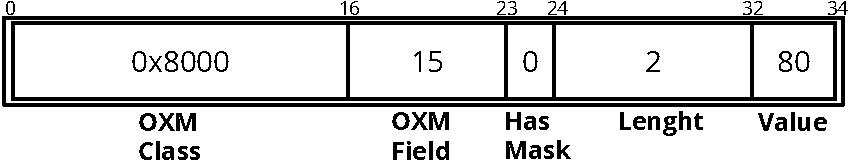
\includegraphics[height=6cm,width=\textwidth,keepaspectratio]{cap4/OXMfieldexample.pdf}
\caption{OXM field example}
\label{fig:oxmfield}
\end{figure}

Some challenges arise with the OXM introduction. Whereas extension of match support for messages is solved, there is nothing concerning the packet parsing in the Datapath. The next subsections discuss how our implementation deals with protocol fields extensibility in the software switch. 

    \subsubsection{Packet Parser}
    \label{pktparser}

    Each new protocol added for the OpenFlow specification demands the addition of specific code to extract the new fields. Distinct protocols may have singular and complex parsing methods. For instance, variable fields such as IP options can require cumbersome deep packet inspection. For this reason, the Packet Parser implementation needs to be flexible and easy to extend. Also, the idea of simple insertion of new match fields meets the ease of extension requisite.    
    
    As a means to achieve a Packet Parser implementation featuring the mentioned characteristics, we have come up with a design which uses a packet description language to assist the parsing. Figure \ref{fig:netbee} shows the Packet Parser model implemented on the switch Datapath. Each module is described as follows:
    
    \begin{figure}[h]
    \centering
    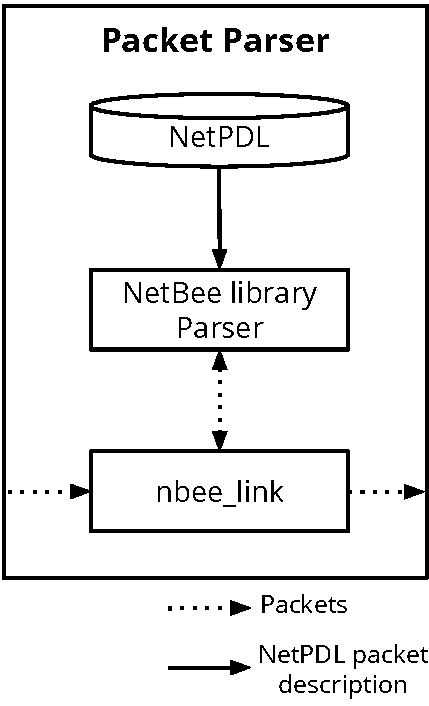
\includegraphics[height=9cm,width=\textwidth,keepaspectratio]{cap4/PacketParserEngine.pdf}
    \caption{Packet Parser components}
    \label{fig:netbee}
    \end{figure}
    
    \begin{itemize}
    \item \textbf{NetPDL}. The Network Protocol Description Language (NetPDL)\cite{Risso:2006:NEX:1141112.1141119} is the packet description language. It is a XML-based language and has a large number of protocols and specified encapsulations. In addition, the simple language definition, allows easy and fast addition of non available protocol description. An example of how the UDP protocol is described using NetPDL can be foung in the Annex \ref{annex:NetPDLdesc}. In the Figure \ref{fig:netbee} the NetPDL module feeds the parsing library with the description of the OpenFlow 1.3 supported match fields.
    
    \item \textbf{NetBee library Parser}. Netbee is as library for packet processing \cite{nbee}. It is composed by several modules for different types of network application, such as packet filtering and sniffing. For our Packet Parser implementation, we use the Netbee library decoding objects. This objects come from a C++ set of classes and methods that ease packet decoding. To accomplish this, firstly Netbee loads the NetPDL protocols specification into the machine Random Access memory (RAM) and on a packet. Then, received packets are decoded according to the NetPDL description and and the extracted information are stored in a protocol tree. Finally, packet field values can be retrieved from the tree using specific methods of the library. 
    
    \item \textbf{nbee_link}. This module is where packets are converted in the flow match structure. Arriving packets are sent for the Netbee library for decoding. From the protocols tree generated by Netbee, the nbee_link module   
extracts the field values and builds the packet match structure that will be sent to the Flow Table look up. The code to extract a protocol is shown by Listing \ref{nbeeparsing}. Using the Netbee method \textit{GetPDMLField}, we get the three ethernet protocol supported fields in OpenFlow 1.3. The second argument of \textit{GetPDMLField} reflects the field name defined in the NetPDL specification. The function \textit{nblink_extract_proto_fields} receives the extracted field value and type and inserts this into the match structure. Another important piece of code is present in the third line. For possible further processing, for instance, the application of a \textit{set field} action, a reference to the protocol position needs to is stored. 
    \\
    \begin{lstlisting}[caption={Ethernet parsing in the nbee_link module}, label=nbeeparsing,]
    if (protocol_Name.compare("ethernet") == 0 && pkt_proto->eth == NULL)
    {
        pkt_proto->eth = (struct eth_header *) ( (uint8_t*) pktin->data + proto->Position);
        PDMLReader->GetPDMLField(proto->Name, (char*) "dst", proto->FirstField, &field);
        nblink_extract_proto_fields(pktin, field, pktout, OXM_OF_ETH_DST);
        PDMLReader->GetPDMLField(proto->Name, (char*) "src", proto->FirstField, &field);
        nblink_extract_proto_fields(pktin, field, pktout, OXM_OF_ETH_SRC);
        PDMLReader->GetPDMLField(proto->Name, (char*) "type", proto->FirstField, &field);
        nblink_extract_proto_fields(pktin, field, pktout, OXM_OF_ETH_TYPE);
    }
    \end{lstlisting}      
    
    \end{itemize}
    
    An example of how helpful is a flexible design for the Packer Parser is on the support for IPv6 Extension Headers (EH) \cite{rfc2460}. EHs parsing execution is not a trivial task, as there are different types and formats. What is more, IPv6 packets may present complex combinations of headers. In OpenFlow 1.3 support for IPv6 EHs is not based in values, but in a special bitmap that matches in the presence of EHs. Besides, a bit field to matches an IPv6 packet only if their EHs are in the recommended order. All of these details would result in a large ammount of code to parse EHs correctly, however, it is done in few lines, due to our extensible implementation and the NetPDL language.    
    \subsubsection{Flow Match Prerequisites}
    
    Another change brought by OXMs is the introduction of flow match fields prerequisites. In order to obtain flow match consistency, some match fields require the presence of other fields. For example, matching any ARP protocol field requires the ethertype field having the correct value for an ARP packet. Thereby, inconsistent flows are denied by the Flow Table.  
      
    To map OXM fields prerequisites, a file \footnote{This file was inpired by the old way that OVS handled the Nicira Extended Match (NXM) format. NXM is the format that gave origin to OXM.}, with several C Preprocessor macros, was created. The macros map each field with their respective network layer 2, layer 3 or upper level requisite. In addition there is also a field that tells if a field is maskable or not. Listing \ref{oxmrequisite} shows prerequisites and fields macros definition. Also, it gives an example of a field created by the \textit{DEFINE_FIELD} macro. 
\\
\begin{lstlisting}[caption={Ethernet parsing in the nbee_link module}, label=oxmrequisite,]

#define OXM_DL_NONE   (0, 0)
#define OXM_DL_ARP    (ETH_TYPE_ARP, 0)
#define OXM_DL_PBB    (ETH_TYPE_PBB,0)
#define OXM_DL_IP     (ETH_TYPE_IP, 0)
#define OXM_DL_MPLS   (ETH_TYPE_MPLS, ETH_TYPE_MPLS_MCAST)
#define OXM_DL_IPV6   (ETH_TYPE_IPV6, 0)
#define OXM_DL_IP_ANY (ETH_TYPE_IP, ETH_TYPE_IPV6)

#define DEFINE_FIELD_M(HEADER,  DL_TYPES, NW_PROTO, MASKABLE)  \
    DEFINE_FIELD(HEADER,  DL_TYPES, NW_PROTO, MASKABLE)        \
    DEFINE_FIELD(HEADER##_W, DL_TYPES, NW_PROTO, true)

DEFINE_FIELD    (OF_TCP_SRC,        OXM_DL_IP_ANY,   IPPROTO_TCP,    false)

\end{lstlisting}   

    OXMs matches definitions are loaded by the Oflib, and used in the function \textit{oxm_pull_match}, which is called during the match unpack. Among the tests performed to detect invalid OXM fields are: bad prerequisite, duplicate fields, wrong masked and nonexistent field.  

    \subsubsection{Flow Matching}
    
    In the pursuit for the best way to perform flow matching inside the flow table, developers might want to try different algorithms and data structures. For this reason, the switch implements a flexible and easy interface to change the way packets are matched. 
    
    Match fields are part of the software switch \textit{flow_entry} struct. Instead of defining a fixed match as one of the \textit{flow_entry} member, a pointer to Oflib \textit{struct ofl_match_header} is left as a reference for the entry match fields. Therefore, if a developer wants to experiment his own match structure, there is only the need to make it start with an \textit{ ofl_match_header}.    

    This work presents a default flow matching using the Oflib match structure called \textit{ofl_match}. Besides the match header, the struct includes a Hash Map structure to store OXM TLVs. Each OXM entries in the Hash Map has an  exclusive key, created by the combination of the field Type and Length information. Storing only flow specified fields saves memory space, at a small cost of the pointers created to mantain the data structure. Another advantage in the Hash Map use in the match structure is the constant access time for the OXMs. Fast element access is very important for two of the most common operations:
    
    \begin{itemize}
    \item \textbf{Check packet matching}. Packet fields are extracted and matched against the flows. Matching is performed by look ups of the packet fields in the Hash Map.        
    
    \item \textbf{Check flow collision}. Flows collide when a new flow is installed and the Flow Table contains a flow with the same match fields and priority. In this case the old one is replaced by the new one. The Hash Map allows a direct comparison of fields.
    \end{itemize}

    Another detail about flow matching in the software switch is about the linear behavior of Flow Table look up. The Flow Table stores flows in a list ordered by priority. When a packet is sent to the flow match it loops through the flow list until finding a matching rule or reach its end. This is the most simple approach for the flow match and was chosen for its simplicity. Developers who might want to modify the behaviour of Flow Table look up just need to add their own code for the function \textit{flow_table_lookup}.
         
    \subsubsection{Extensible context expression in ’packet-in’}
    
    Former \textit{packet-in} message contained little information about the packet parsed in the Datapath. The only match field present was the switch input port. In order to get the other packet fields a controller needs to parse the packet header, included in the end of \textit{packet-in}. This causes an unnecessary parsing repetition in the control plane. With the OXM introduction, OpenFlow 1.3 solves this problem sending the extracted packet fields in the form of OXMs, making it easier for the control plane to retrieve the packet fields.  
    
    While an standard switch implementation requires only context information, which are input port, metadata and tunnel_id, our implementation follows the option to add all parsed fields in a \textit{packet-in} message.    

\subsection{Set Field action}
\label{sec:sec43}    

Support for rewriting packet fields exists since the first OpenFlow version. However, it was limited to a small set of fields. In OpenFlow 1.3, with the OXM introduction, a \textit{flow mod} message can carry a  \textit{set field} action with any of the OXMs defined by the specification. It is up for the switch designers to decide which fields are allowed for overwrite.   

Implementation of \textit{set field} is a little bit tricky, as the consistence is achieved through the match fields. For instance, a flow with a \textit{set field} action to rewrite the IP source address, needs to present in the match fields the same ethertype - 0x800 in hexadecimal - of the IP protocol. How the pack and unpack of match fields and actions is performed by different functions, needs to be checked in the Datapath. When handling a new \textit{flow mod} message, the Flow Table calls the function \textit{dp_actions_check_set_field_req}. This function uses an Oflib function to check if the prerequisites are ok and validate the action.

Another frequent task caused by rewriting fields is protocol CheckSum recalculation. Fields like the IP source and destination, in the case of change, requires recalculation of IP and TCP CheckSum values. Fortunately these protocols CheckSum calculation is very simple \cite{rfc1071}. This is not the case for the SCTP protocol \cite{rfc3309}. SCTP CheckSum is calculated using a Cyclic Redundancy Check (CRC). In order to recalculate the SCTP CheckSum value we used a Python program named pycrc \footnote{pycrc v0.8.2, Available at http://www.tty1.net/pycrc/}. The program takes as input the CRC polynomial and generates all the functions necessary for the calculations. Listings \ref{set_field} shows the code to rewrite the SCTP destination port. In the packet field rewriting we attribute a pointer to the protocol struct representation to the packet position obtained by the Packet Parser. Doing so, we can easily change the current value of the action value.
\\
\begin{lstlisting}[caption={Ethernet parsing in the nbee_link module}, label=set_field,]
case OXM_OF_SCTP_DST:{
                crc_t crc;
                struct sctp_header *sctp = pkt->handle_std->proto->sctp;                
                size_t len = ((uint8_t*) ofpbuf_tail(pkt->handle_std->pkt->buffer)) - (uint8_t *) sctp;
                uint16_t v = htons(*(uint16_t*) act->field->value);
                sctp->sctp_csum = 0;
                memcpy(&sctp->sctp_dst, &v, OXM_LENGTH(act->field->header));
                crc = crc_init();
                crc = crc_update(crc, (unsigned char*)sctp, len);                            
                crc = crc_finalize(crc);
                sctp->sctp_csum = crc;
                break;        
            }
\end{lstlisting}  

\subsection{Per-flow Metering}

    The Meter Table implementation follows the architectural details and responsibilities of the element described on section \ref{sec:MeterTable}.
Firstly we defined a structure for the Meter Table. The main components are the table features, such as the max number of entries and supported band types, and a Hash Map of meter entries. Other members include a reference pointer to the Datapath, allowing a Meter Table to call the function to send OpenFlow messages; and two counters: one for the number of meter entries and another one for the quantity of bands. Secondly, we implemented a set of functions: init and destruction of the Meter Table; \textit{meter mod} and \textit{meter features} messages handlers; find and apply a meter entry.

    Structures of meter entries are composed of a configuration, which contains information about the meter id and meter bands, and a struct for recording statistics. In addition, the meter entry has pointers to the Datapath and the Meter Table, similar to what is done in the Meter Table struct. Finally, it has a list of flow references. If the meter entry is deleted, all flows that send packets to the meter entry are deleted. 

    Meter entry bands are chosen accordingly to a configured rate - in Kilo packets (Kpps) per second or Kilobits per second (Kbps). Thus, it is necessary to measure the flow matched packets in function of one of the specified unities. The first idea to implement rate measuring scheme, considered the use of matched flow counters, divided by the number of matched bytes by some time interval. Although easy to implement, this approach proved inaccurate after some attempts to limit the bandwidth between two hosts connected to the switch.  
    
    After a better analysis of the task and some literature research we found and implemented a simple and efficient algorithm used for rate policy: the Token Bucket \cite{Tanenbaum:2002:CN:572404}. Figure \ref{fig:tokenbucket} illustrates how the Token Bucket works within a meter band. Basically each meter band has a bucket attached to it. At every second the bucket is refilled with a numbers of tokens equal to the meter rate. When a packet is sent to the Meter Table, it goes through each band bucket belonging to the meter entry. Inside the bucket, packets consume a number of tokens equal to their size. If there are enough tokens, the OpenFlow pipeline continues processing the packet, otherwise, the meter band is chosen and executed.               

    \begin{figure}[h]
    \centering
    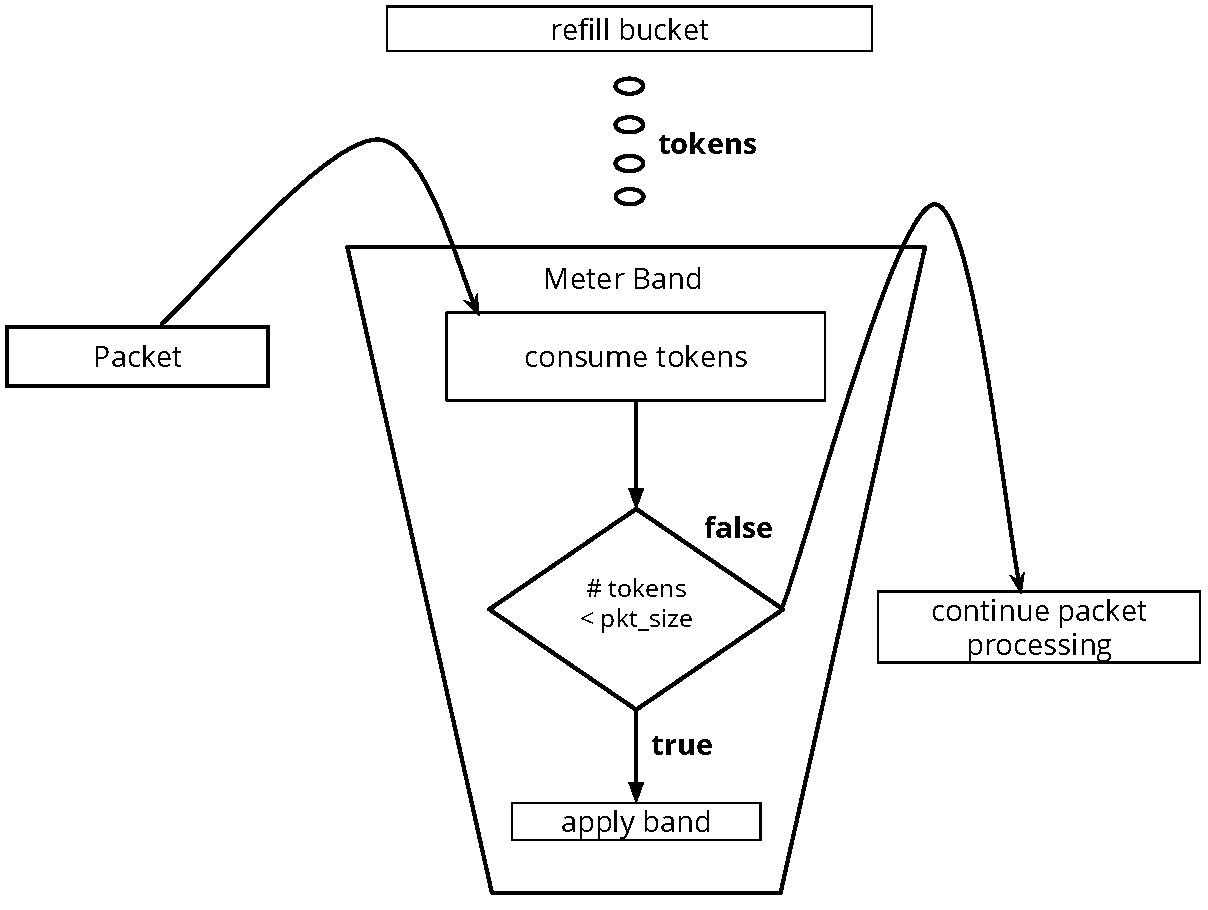
\includegraphics[height=9cm,width=\textwidth,keepaspectratio]{cap4/TokenBucket.pdf}
    \caption{Token Bucket Algorithm illustration inside the meter band}
    \label{fig:tokenbucket}
    \end{figure}

\label{sec:sec44}

\subsection{Connection Features}
\label{sec:sec45}

    Network control protocols must be designed with scalability and high availability on mind. Node failures and high traffic loads may cause frustration for early adopters of new technologies, as these two important points usually are not considered by initial versions. Previous OpenFlow versions fall into this category of protocols, criticized by the lack of mechanisms to handle control plane issues. 
    
    More recent OpenFlow versions try to address control plane scalability and high availability with the addition of new features for OpenFlow connections. Auxiliary connections allow higher scalability for message exchanging, while controller roles try to enable fast failover for OpenFlow controllers. Event filtering, in turn, may be seen as a mechanism that sum up on these two topics. In the next subsections we will see a more detailed description of each feature and how they have been implemented in our software switch.
    
    \subsubsection{Auxiliary Connections}
    
    Auxiliary connections allow a controller to create more than one Communication Channel with a single switch. These connections add the possibility to exploit message parallelism and create a channel for specific types of messages. For instance, a controller can use one connection only for \textit{packet-in} messages. 
    
    As a proof-of-concept we have implemented basic support for auxiliary connections. In our implementation, there is support for only one additional channel and it only carries \textit{packet-in} messages. The following items show steps added in the switch code to handle auxiliary connection.
    
    \begin{itemize}
    \item The software switch sends OpenFlow messages, for the Communication Channel, encapsulated into a struct called \textit{ofbuf}. The struct is a buffer that holds information such as the pointer for the first allocated byte and the size of bytes in use. In order to identify which connection is being used to receive or send the message, we have added a new member called \textit{conn_id}. The possible values for \textit{conn_id} are MAIN_CONNECTION and PTIN_CONNECTION.  
    
    \item A new connection listener was added to the Datapath. If an auxiliary connection is specified when running the datapath, the auxiliary listener is opened after the main connection listener.
    
    \item When the Datapath talks to remotes, it searches for the auxiliary connection. If the connection exists, it processes messages received by the connection.
    
    \item On sending OpenFlow messages, the switch by default maps to the MAIN_CONNECTION. If the message is a reply from  a sent message of a sender connection, the connection id is set to the same id used by the sender. In the last case, if the message type is a \textit{packet-in}, the switch uses PTIN_CONNECTION for the connection id. 
    
    \end{itemize}
    
    The start an auxiliary connection from one controller is disabled by default in our software switch standard program execution. To enable auxiliary connections a user should specify the \textit{multiconn} option in the command line option   

    \subsubsection{Controller Role}

    Controller Role is a mechanism to permit connection of multiple controllers with different duties. One of the possible use cases of roles is for fast failover, in which when the main controller goes down, a backup controller assumes the switch command. There are three possible roles for controllers: Master, Slave and Equal. A master controller has permissions to send and receive any type of OpenFlow messages. Slaves have very strict default permissions, allowed only to receive a specific set of messages. The last role, Equal, is the default role when a controller connects to the switch and the other controllers connected do not have a defined role.
    
    Role election is totally driven by the control plane, however some additional code is required for the switch. In order to implement controller role support in our software switch we first filtered asynchronous messages received by Slave controllers. Then we restricted slaves to send only read state messages, for example, \textit{flow stats} and \textit{table stats}. The last insertion is the algorithm defined by the specification to handle the \textit{role request} generation_id. Messages with a generation id smaller than previous generation ids seen by the switch are discarded. Listing \ref{rolegenid} presents the function that implements the algorithm.
\pagebreak
\begin{lstlisting}[caption={Ethernet parsing in the nbee_link module}, label=rolegenid,]
static ofl_err
dp_check_generation_id(struct datapath *dp, uint64_t new_gen_id){

    if(dp->generation_id >= 0  && ((uint64_t)(new_gen_id - dp->generation_id) < 0) )
        return ofl_error(OFPET_ROLE_REQUEST_FAILED, OFPRRFC_STALE);
    else dp->generation_id = new_gen_id;
    return 0;
}
\end{lstlisting} 
    \subsubsection{Event Filtering}

    Event Filtering enables controllers to filter undesired asynchronous messages, sent by the switch. Filtering of asynchronous messages is possible for three types: \textit{port status}, \textit{packet-in} and \textit{flow removed}. In addition, a controller can also choose to not receive these message types for the generation reason. For example, a \textit{packet-in} can be generated by an action to output the packet for the controller. This feature, along with auxiliary connections, gives power for controllers to create exclusive message channels.
    
    Message filtering is handled by the Datapath. On a \textit{set async request}, the Datapath sets the controller remote channel with bitmaps values sent in the message defined by the OpenFlow 1.3 specification, shown on Listing \ref{asyncmessage}. Each bit set in the bitmap represents a message type and a reason. For instance, a bit with value 4 in \textit{flow_removed_mask[0]}, determines if the controller will receive \textit{flow removed messages} with reason OFPRR_DELETE when the role is Master.  
    
    Filtering happens before the sending of an OpenFlow message. The Datapath function to send an OpenFlow buffer through the Communication Channel checks the remote configuration and the type of the message to be sent. If it is one of the three asynchronous messages and the reason and the controller roles matches the remote filtering configuration, the message is dropped. 
    
\begin{lstlisting}[caption={Ethernet parsing in the nbee_link module}, label=asyncmessage,]    

/* Asynchronous message configuration. */
struct ofp_async_config {
    struct ofp_header header;
    /* OFPT_GET_ASYNC_REPLY or OFPT_SET_ASYNC. */
    uint32_t packet_in_mask[2];
    /* Bitmasks of OFPR_* values. */
    uint32_t port_status_mask[2]; /* Bitmasks of OFPPR_* values. */
    uint32_t flow_removed_mask[2];/* Bitmasks of OFPRR_* values. */
};
OFP_ASSERT(sizeof(struct ofp_async_config) == 32);

\end{lstlisting}

\subsection{Other Changes}
\label{sec:sec46}

There is a complete list of other changes we have made to upgrade the base software switch from OpenFlow 1.1 to OpenFlow 1.3. Whereas these other changes are important the implementation demanded less effort than changes described in the previous subsections. For this reason, we will list and comment them briefly:

\begin{itemize}
\item \textbf{Table Miss.} Previous behavior of OpenFlow switches on non matching packets were defined by configuration flags. OpenFlow 1.3 removes these flags and defines table-miss flow entry. This entry is an all field matching with the lowest possible priority. Table miss support implementation required the remotion of code to handle the old behavior. In addition, in the case of a table-miss entry with an action to output the packet for the controller, the switch sends the \textit{packet-in} message with a reason of type \textit{OFPR_NO_MATCH}.      

\item \textbf{Rework Tag Order.} The order of the supported protocols tags, pushed by an OpenFlow action, was dictated by the specification. In OpenFlow 1.3, tags do not have a right order and should be pushed in the outermost possible position. In the code, these features were reflected by deletion of old restrictions and right adjustment of the tag order. 

\item \textbf{Addition of MPLS BOS and PBB fields.} The MPLS Bottom of the Stack (BOS) field and support for the Provider Backbone Bridge Protocol (PBB) was quite easy to implement thanks to the Packet Parser design, described in the subsection \ref{pktparser}. PBB support also included actions to push and to pop tags in a packet. These actions are similiar to MPLS and VLAN push and pop, thus implementation for PBB followed a workflow similar to the mentioned protocols.  

\item \textbf{Duration for stats.} Old versions included the time of existence  only for flow entries statistics. OpenFlow 1.3 introduces a duration field for meter, port, queue and group statistics and they are supported by the software switch.  

\end{itemize}

\subsection{Dpctl}
\label{sec:sec47}

Dpctl is a useful tool for management and debugging of the tables of a single OpenFlow. By using Dpctl, it is possible to avoid addition of debugging code in a controller application, for example, query the current Flow Table state. Available since the OpenFlow 1.0 reference implementation, we find its upgrade quite necessary to help during our switch development. 

To connect with Dpctl, the software switch keeps a passive listening port. Unlike the switch active sockets, which looks for a controller to connect, the passive port waits for a connection. Thereby, Dpctl must initiate an active connection in order to establish contact with the switch. The switch port number for incoming connections is 6634.

Several changes were required in order to upgrade Dpctl for OpenFlow 1.3. New commands had to be implemented for meter, table stats and features, along with new arguments for existing commands, like flow mod, such as instructions and recently modified or added match fields. As each command sends a different message for the switch, the independence of Oflib comes in handy for this tasks.  

Dpctl uses OFlib to create and receive switch messages and also to print their contents. After command parsing, the arguments are stored in the respective OFlib structures, for example, a \textit{meter-mod} command creates the \textit{struct ofl_msg_meter_mod}. The struct is packed using the Oflib function and then sent for the switch. Commands like \textit{stats-flow} always generate an answer, which on receipt are unpacked by Oflib and the results are displayed on the screen. Check for message delivery on Dpctl  accomplished through the use of OpenFlow barrier messages. After every message a barrier is sent for the switch to confirm the receipt.


\section{Open source development}
\label{OpenSourceDev}

An important aspect about the software switch development is the project open source nature. The code is distributed under the BSD 3-clause license, a permissive license with few restrictions about software redistribution. This type of license fits with our main motivation, because it gives freedom to use and encourages collaboration. 

The code is available on GitHub \footnote{Project Page: https://github.com/CPqD/ofsoftswitch13}, a well known web site for projects that adopt git \cite{GIT} as the source control management tool. Git is ideal for distributed development, as developers keep a local copy of the current code state and usually make changes to local branches. These changes are tested, reviewed and then merged into main, typically named master branch.    

In this section we will show how this model works in our development process and show how it helps in the process of code maintenance and support.    

\subsection{Development workflow}

GitHub is a very social platform and leverages code collaboration for open source projects. For this reason, code development follows a very simple and common workflow for public git projects hosted at GitHub:

\begin{itemize}

\item Developers fork the code and create local branches of new features or fixes. 

\item Changes are made in the branch and committed.

\item A Pull Request is sent to the main repository.  

\item Code is reviewed and tested. 

\item Changes are merged into master.

\end{itemize}

This steps enabled collaboration of developers from all around the world. Also, this work model adds transparency to the development, allowing anyone from the community to track changes, enhancements and bugs. The last benefit is fairness, as every git commit is signed with the author name, credits are guaranteed to be given and shown for all contributors.          

\subsection{Code maintenance}
\label{CodeMaintenance}

In traditional Waterfall model, software life cycle maintenance is an independent phase and comes after implementation and testing steps \cite{Ruparelia:2010:SDL:1764810.1764814}. While this development model is well suited for large and well defined projects, it lacks flexibility and the dynamism required for an open source project that demands fast reactions to bugs and inquires for enhancements. Therefore, maintenance and support are processes that walk side by side with implementation and test. 

The most common of maintenance tasks are usually triggered by users requests on GitHub issue tracker. Users are free to open tickets asking for enhancements or to report bugs. The issue tracker is also a common place for questions about the software switch code or execution. Thus, maintenance and support are very close in the switch development.          

Another important aspect of code maintenance are regression tests. After every new feature implemented or issue fixed, we run tests frameworks presented in section \ref{sec:testemulation}, ensuring that no change caused a break in functional code. Furthermore, Ryu tests run automatically after a new commit, since their developers keep an infrastructure to detect changes, execute the tests and publish results on a public web page \footnote{Ryu Certification - http://osrg.github.io/ryu/certification.html}. 

The idea of feature testing gives light for possible evolution in our development model. A Test Driven Development (TDD) \cite{Nagappan:2008:RQI:1380662.1380664}, a development approach where tests are written first, before the software functionalities. A TDD based methodology would force continuous maintenance in the code, because developers, when designing tests, are already thinking about the system behavior and how it going to be used and. Moreover, they might preview further changes. Thus, leading to implementation of more maintainable code. 

One possible parallel with TDD,  is the ONF Extension Working Group. This group is responsible for suggestion and validation of new OpenFlow features. Functionality approval process goes through proposal and test implementation in some of the available OpenFlow software switches. This can be seen as the test design phase of TDD. After validation, i.e running the test and confirm it is working, the feature is ready to be written in the specification, just like code ready for production.                 




 
\chapter{Evaluation}
\label{cap:cap05}

In this chapter we evaluate our work in terms of the requisites presented on section \ref{sec:sec02}. The first section shows in numbers how many features are covered by the software switch. Following, in the next section, we present the results of performance benchmarks tests. The last chapter section is a qualitative evaluation about the code ease to change. We will highlight some known examples that demonstrate the software switch code simplicity.      

The software switch evaluated version dates from the last commit pushed to GithHub. The box below shows the dates and last code changes description.

\begin{framed}

\begin{itemize}
\item \textbf{commit} cb740bd2565ac7e5d61ebe30ee75160a5452a033
\item   \textbf{Commit:}     Eder Leão Fernandes <ederleaofernandes@gmail.com> 
\item \textbf{CommitDate:} Mon Feb 23 18:42:49 2015 -0300 
\end{itemize}
     
    Add flags member to ofp_flow_stats.
    
    Fix missing flags field in the response of a flow stats request.
\end{framed}

\section{Feature Completeness}
\label{sec:FeatureComplete}
Evaluate the proper operation of the OpenFlow switch features is not a trivial task because of multiple and rich configurations allowed by the specification. For example, test all flow match fields combination would require creation of a large number of flows and packets, making manual tests very time consuming. For this reason, automatic tests frameworks, discussed on section \ref{sec:testemulation}, are the best options to test the switch functionality in order to evaluate features completeness.    

OFTest and Ryu Certification are the two test frameworks used for switch validation. As mentioned in chapter \ref{CodeMaintenance}, both are important tools for the software switch development. While Ryu certification has a strong focus on validation of the Datapath, OFTest offers a nice set of test cases for control and data plane message exchange. In the next sections we present a resume of the results obtained.  


\subsection{OFTest results}

Testing in OFTest is simple as it provides scripts in Python to run the switch and the test cases. Each test case starts a controller which connects with a running switch, executes the test instructions and checks the switch answers. 

Some controller to switch, like a \textit{flow stats} request, and symmetric messages demand an answer from the switch. Thus, the main purpose of the framework usage with the software switch is for message handling validation. Although, OFTest has capabilities to evaluate the pipeline processing - for instance, checking if a packet was correctly forwarded by a flow - we found in Ryu a more comprehensive test set for this task. 

Table \ref{tab:oftestbasic} shows test results for basic OpenFlow messages. The major type of messages of the the test set are messages to query information about the state of manifold switch elements, such as \textit{GroupFeatureStats} and \textit{MeterStats}. Also, there are some configuration messages, like the \textit{PortConfigMod}. In all tests the switch returned the right answer for the control plane.


\begin{table}[h]
\centering
\caption{Basic OpenFlow messages}
\label{tab:oftestbasic}
\begin{tabular}{|l|l|l|l|l|}
\cline{1-2} \cline{4-5}
\multicolumn{1}{|c|}{\textbf{Message}} & \textbf{Result} &  & \textbf{Message}   & \textbf{Result} \\ \cline{1-2} \cline{4-5} 
AggregateStats                         & ok              &  & GroupFeaturesStats & ok              \\ \cline{1-2} \cline{4-5} 
AsyncConfigGet                         & ok              &  & GroupStats         & ok              \\ \cline{1-2} \cline{4-5} 
DescStats                              & ok              &  & MeterConfigStats   & ok              \\ \cline{1-2} \cline{4-5} 
Echo                                   & ok              &  & MeterFeaturesStats & ok              \\ \cline{1-2} \cline{4-5} 
EchoWithData                           & ok              &  & MeterStats         & ok              \\ \cline{1-2} \cline{4-5} 
FeaturesRequest                        & ok              &  & QueueStats         & ok              \\ \cline{1-2} \cline{4-5} 
FlowStats                              & ok              &  & PortConfigMod      & ok              \\ \cline{1-2} \cline{4-5} 
FlowRemoveAll                          & ok              &  & PortDescStats      & ok              \\ \cline{1-2} \cline{4-5} 
GroupDescStats                         & ok              &  & TableStats         & ok              \\ \cline{1-2} \cline{4-5} 
\end{tabular}
\end{table}

Controller roles test results are shown in table \ref{tab:oftestrole}. This tests checks if the software switch changes correctly controller roles and if the respective permission police is respected. As in the previous message tests, all role tests were sucessful.    

\begin{table}[h]
\centering
\caption{Role request message results}
\label{tab:oftestrole}
\begin{tabular}{|l|l|}
\hline
\textbf{Role Request Tests} & \textbf{Results} \\ \hline
RoleRequestEqualToSlave     & ok               \\ \hline
RoleRequestSlaveToMaster    & ok               \\ \hline
RolePermissions             & ok               \\ \hline
RoleRequestEqualToMaster    & ok               \\ \hline
RoleRequestNochange         & ok               \\ \hline
SlaveNoPacketIn             & ok               \\ \hline
\end{tabular}
\end{table}

\subsection{Ryu Certification results}

The Ryu Certification tests are divided into five categories: Action, Set-Field, Match, Group and Meter. The test sets of each category are very comprehensive, with tests for different packet types.

Table \ref{tab:ryuresults} is a resume of test results - the complete list of test cases can be found on Annex \ref{annex:ryucert}.  - for this work compared to the other three switches presented on chapter \ref{cap:cap02}. White cells give the number of tests passed, while grey cells show the number of test cases that returned an error. Tests are divided by each category, with the last two columns giving the total sum of working and non working features. The first row presents the results for this work. \footnote{ofsoftswitch13 is the software switch repository} 

% Please add the following required packages to your document preamble:
% \usepackage{graphicx}
% \usepackage[table,xcdraw]{xcolor}
% If you use beamer only pass "xcolor=table" option, i.e. \documentclass[xcolor=table]{beamer}
\begin{table}[h]
\centering
\caption{Ryu Certification results comparison}
\resizebox{\textwidth}{!}{%
\begin{tabular}{|l|ll|ll|ll|ll|ll|ll|}
\hline
\textbf{Switch}       & \multicolumn{2}{l|}{\textbf{Action}} & \multicolumn{2}{l|}{\textbf{Set-Field}} & \multicolumn{2}{l|}{\textbf{Match}} & \multicolumn{2}{l|}{\textbf{Group}} & \multicolumn{2}{l|}{\textbf{Meter}} & \multicolumn{2}{l|}{\textbf{Total}} \\ \hline
\textbf{ofsoftswitch13} & 50    & \cellcolor[HTML]{9B9B9B}6    & 159    & \cellcolor[HTML]{9B9B9B}7      & 708  & \cellcolor[HTML]{9B9B9B}6    & 15   & \cellcolor[HTML]{9B9B9B}0    & 30   & \cellcolor[HTML]{9B9B9B}6    & 848  & \cellcolor[HTML]{9B9B9B}25   \\ \hline
\textbf{Open vSwitch} & 34    & \cellcolor[HTML]{9B9B9B}22   & 96     & \cellcolor[HTML]{9B9B9B}74     & 534  & \cellcolor[HTML]{9B9B9B}180  & 0    & \cellcolor[HTML]{9B9B9B}36   & 0    & \cellcolor[HTML]{9B9B9B}36   & 670  & \cellcolor[HTML]{9B9B9B}321  \\ \hline
\textbf{LINC}         & 24    & \cellcolor[HTML]{9B9B9B}32   & 68     & \cellcolor[HTML]{9B9B9B}102    & 428  & \cellcolor[HTML]{9B9B9B}286  & 3    & \cellcolor[HTML]{9B9B9B}12   & 0    & \cellcolor[HTML]{9B9B9B}24   & 523  & \cellcolor[HTML]{9B9B9B}456  \\ \hline
\textbf{Trema}        & 50    & \cellcolor[HTML]{9B9B9B}6    & 159    & \cellcolor[HTML]{9B9B9B}11     & 708  & \cellcolor[HTML]{9B9B9B}6    & 15   & \cellcolor[HTML]{9B9B9B}0    & 34   & \cellcolor[HTML]{9B9B9B}2    & 852  & \cellcolor[HTML]{9B9B9B}25   \\ \hline
\end{tabular}
}
\label{tab:ryuresults}
\end{table}

Results show that the software switch has a higher number of working features than Open vSwitch and LINC. With only 25 errors, it is tied with Trema in the number of supported features. There is a small difference between ofsoftswitch13 and Trema, in the total number of tests passing. This happens because Ryu Certification does not execute four tests due to old switch restrictions.

The values presented in this section are from the official certification site \footnote{http://osrg.github.io/ryu-certification/switch/config/ofsoftswitch13.html}. Some failed test results presented on the site work in our internal test setup. For instance, matching on \textit{PBB ISID} value. However, we chose to show the official results as we could not identify the causes for different results. In addition, some test may never pass. For example, \textit{IP proto} modification causes packet malformation, because the IP proto packet field will not conform with the next layer protocol, which leads to a test failure. 

\section{Performance Benchmarks}

One of the software switch requirements listed on chapter \ref{cap:intro} is to reach a maximum throughput of at least 100 Mb/s. For this reason we evaluated the switch performance in terms of network metrics. In this section we show how the switch performs for different packet sizes in comparison with other userspace software switches. Also, we investigated how performance is affected by the number of flows and by the number of tables traversed to match a packet.  

The machine configuration used to perform measurement tests are listed in the box below. 

\begin{framed}

\begin{itemize}
\item \textbf{Processor}:	8x Intel(R) Core(TM) i7-2670QM CPU @ 2.20GHz
\item \textbf{Memory}:	6003MB 
\item \textbf{Operating}: System	Ubuntu 14.04.2 LTS
\end{itemize}

\end{framed}

    \subsection{Maximum Throughput}
    \label{sec:MaxBand}
    This test evaluates the maximum forwarding rate the software switch can reach in comparison to other userspace implementations. 
    
    The setup for maximum throughput evaluation is the following:
    
    \begin{itemize}
    \item A running instance of the software switch with two virtual interfaces - Port 1 and Port 2 - attached. 
    \item One flow installed in the flow table to match a packet sent to Port 1 with destiny ethernet 00:00:00:00:01. The action is output packet to Port 2. 
    \item A packet traffic generator. We used a simple program named packeth \cite{packeth}.
    \item A script running in the linux terminal checking the current packet rate on Port 2.   
    \end{itemize}
    
    The test starts by installing the flow in the switch Flow Table. After, we inject packets, using the traffic generator, directly into Port 1. The bandwidth results of Port 2, reported by the script, are used to calculate the average rate and the standard deviation.  
    Two transmission measurements were made: for small packets of 64Kb and bigger packets of 1500Kb. Figure \ref{graph:comparison} shows results for both experiments.

    \begin{figure}[H]
        \begin{minipage}{\textwidth}
        \centering
        \begin{subfigure}{.7\textwidth}
        \begin{tikzpicture}    
 
         \begin{axis}[
            xtick=data,
            symbolic x coords={ofsoftswitch13, LINC, Trema},
            nodes near coords,
            width= 10cm,
            bar width=1.5cm,
            enlarge x limits={abs=1.2cm},
            ylabel near ticks,
            xlabel near ticks,
            ymin=0,
            ylabel=Throughput (Kpps),
            visualization depends on=-y \as \negy,
            visualization depends on=y \as \y,
            visualization depends on=\thisrow{error} \as \yerror,
            every node near coord/.append style={
                font=\small,
                shift={(0, transformdirectiony(\negy))},
                text width=1.5cm,
                align=center
            },
            nodes near coords={\pgfmathprintnumber{\y} $\pm$ \pgfmathprintnumber[fixed,precision=4]{\yerror}}]
        
        \addplot[ybar,fill=lightgray,error bars/.cd,y dir=both, y explicit]
        table[y error=error] {
            x y error
            {ofsoftswitch13} 38.08 0.17
            {LINC} 26.13 0.18
            {Trema} 166.42 26.57
        };
        \end{axis}
            
         \end{tikzpicture}
            \caption{Comparison using packets of 64 bytes}
            \label{graph:comparison64}
        \end{subfigure}
        \linebreak
        \begin{subfigure}{.7\textwidth}
        \begin{tikzpicture} 
        
          \begin{axis}[
            xtick=data,
            symbolic x coords={ofsoftswitch13, LINC, Trema},
            nodes near coords,
            width= 10cm,
            bar width=1.5cm,
            enlarge x limits={abs=1.2cm},
            ylabel near ticks,
            xlabel near ticks,
            ymin=0,
            ylabel=Throughput (Mbps),
            visualization depends on=-y \as \negy,
            visualization depends on=y \as \y,
            visualization depends on=\thisrow{error} \as \yerror,
            every node near coord/.append style={
                font=\small,
                shift={(0, transformdirectiony(\negy))},
                text width=1.5cm,
                align=center
            },
            nodes near coords={\pgfmathprintnumber{\y} $\pm$ \pgfmathprintnumber[fixed,precision=4]{\yerror}}]
        
        \addplot[ybar,fill=lightgray,error bars/.cd,y dir=both, y explicit]
        table[y error=error] {
            x y error
            {ofsoftswitch13} 260.25 1.67
            {LINC} 280.35 14.18
            {Trema} 843.56 17.70
        };
        \end{axis}
        
        \end{tikzpicture}
            \caption{Comparison using packets of 1500 bytes}
            \label{graph:comparison1500}
        \end{subfigure}
        \end{minipage}
        \caption{User space software switches throughput comparison}
        \label{graph:comparison}
    \end{figure}
  
   Switch forwarding performance for small packets is evaluated in Kilo packets per second (Kpps). Figure \ref{graph:comparison64} shows that ofsoftswitch13 can handle 38.08 Kpps. This result is very 
   far from Trema and approximatelly 32\% more efficient than LINC. Bigger packets are measured in Mega bits per second. Results presented in Figure \ref{graph:comparison1500} show that ofsoftswitch13 and LINC, with rates of 260.25 Mbps 280.35 Mbps respectively, are slower than Trema with a bandwidth of 843.56 Mbps. 
   
    Although Trema overcomes our work in performance, due to optimization like multiple threads, the most important result of this experiment is the software switch maximum throughput found. This value is higher than the value established by the software switch requirements. 
    
    \subsection{Throughput in function of flows and tables}
    \label{sec:bandflows}
    This experiment measured two factors that may affect the software switch performance. One is the number of flows installed in one table. The second is the number of tables traversed until the match.
    
    For this test we used Mininet with the software switch connecting two hosts. Bandwidth is measured through the  Iperf session established between the two hosts. Flow Table setup for the two cases are the following: 
    
    \begin{enumerate}[label=(\Alph*)]
    \item \textbf{Number of flows}. Install a certain amount of flows, with the same priority, that will not match packets. In the end, two flows, with the same or lesser priority than the previous are installed to forward packets between the two hosts.
    \item \textbf{Number of tables}. Flows to send the packet to next table are installed until the penultimate  table. Then, in the last table install two flows to forward the traffic between the hosts.
    \end{enumerate}
    
        \begin{figure}[H]
            \begin{minipage}{\textwidth}
            \centering
        \begin{subfigure}{.45\textwidth}
            \begin{tikzpicture}
            \begin{axis}[
                xlabel={Number of flows},
                ylabel={Throughput (Mb/s)},
                ymajorgrids=true,
                grid style=dashed,
                ylabel near ticks,
                nodes near coords,
                scale only axis,       
                width=.9\textwidth,
                xlabel near ticks,
                xtick={2, 1024, 2048, 3072, 4096},
            ]
            \addplot[color=black, mark=square,error bars/.cd,y dir=both, y explicit]
            coordinates {
                (2, 156.24) +- (0.00, 4.64709)
                (1024, 88.93) +- (0.00, 1.20467)
                (2048, 64.58) +- (0.00, 0.65115)
                (3072, 46.28) +- (0.00, 0.4492)
                (4096, 38.8) +- (0.00, 0.52493)
            };
            \end{axis}
            \end{tikzpicture}
            \caption{Throughput per number of flows in one table}
            \label{graph:nflows}
        \end{subfigure}
        \hfill
        \begin{subfigure}{.45\textwidth}
            \begin{tikzpicture}
            \begin{axis}[
                xlabel={Number of tables},
                ylabel={Throughput (Mb/s)},
                ymajorgrids=true,
                grid style=dashed,
                ylabel near ticks,
                nodes near coords,
                scale only axis,       
                width=.9\textwidth,
                xlabel near ticks,
                xtick={4, 16, 48, 32, 64},
            ]
            \addplot[color=black, mark=square,error bars/.cd,y dir=both, y explicit]
            coordinates {
                (4, 150) +- (0.00, 3.26599)
                (16, 147.7) +- (0.00, 1.88856)
                (32, 146.5) +- (0.00, 2.36878)
                (48, 144)   +- (0.00, 4)
                (64, 140) +- (0.00, 2.26078)
            };
            \end{axis}
            \end{tikzpicture}
            \caption{Throughput per number of tables}
            \label{graph:ntables}
        \end{subfigure}
        \end{minipage}
            
            \caption{Influence of the number of installed flows on the throughput.}
            \label{graph:scaling}
        \end{figure}     
     
        The graphs in the Figure \ref{graph:scaling} shows that both cases have a strong influence over the switch performance. The most sensitive case is for one table shown in Figure \ref{graph:nflows}, as the number of flows increases the throughput decreases linearly. The increase in the number of tables, shown by the graph in the Figure \ref{graph:ntables}, also causes a linear decrease in the packet rate, however it is smaller than in the first case. These results were already expected, because the software switch implements linear matching. Thus, this experiments were important to verify one improvement point for the software switch.     
     
    \subsection{Ping Round Trip Time}

    Round Trip Time (RTT) is the time between a data request and answer. Several factors might affect the total RTT and and influence network latency. Two examples are the number of nodes between two communicating hosts and the transmission medium. The time a packet takes to enter and leave a switch is also considered for the RTT. Thus, it is important to measure how much the software switch affects the RTT. 
    
    In order to measure the RTT between two hosts connected by our software switch and also LINC and Trema, the following steps are executed:
    
    \begin{enumerate}
    \item Creation of two linux containers (LXC) - Host 1 and Host 2 - with a pair of virtual interfaces \textit{veth0} and \textit{veth1}. LXC is an operating system lightweight virtualization technology, in which is possible to run multiple isolated linux instances as containers. With LXC, we run two containers to serve as the network hosts.    
    \item Execution of a software switch instance of a software switch with the container virtual ports attached on switch interfaces.
    \item Installation of two flows in the switch Flow Table to forward the traffic between the two hosts. 
    \item Configuration of Host 1 and Host 2 with IP addresses in the same network. In our test Host 1 is configured with the IP address 192.168.0.1 and host 2 as 192.168.0.2. 
    \item Execution of the \textit{ping} program in Host 1 to ping the address 192.168.0.2. Ping is a program to send and measure the time between an Internet Control Message Protocol (ICMP) "Echo request" and the ICMP "Echo Reply". The number of Echo requests sent is 100 and the packet sizes are 64Kb.
    \end{enumerate}

    Switch results comparison is shown in Table \ref{pingtable}. This tests give a good approximation for the software switch impact over the network delay, because its connected directly to the hosts. As expected, because of the previous results, Trema is the most efficient among the userspace software switches. The ofsoftswitch13 obtain a low minimum RTT, with 0.304 ms, however the average is approximatelly 1ms. LINC has a very high RTT, with more than a half second to complete. This is not a surprise, because the throughput tests, shown in section \ref{sec:MaxBand}, revealed that LINC does not handle small packets very fast.   
    
    An acceptable RTT value depends on the application running over the network. Latency sensitive programs, like multiplayer online games, benefit from a low RTT. Considering a small network, with not many hops, the RTT in our software switch is acceptable.   

        % Please add the following required packages to your document preamble:
    % \usepackage{graphicx}
    \begin{table}[H]
    \caption{Ping Round Trip Time comparison between software switches}
    \label{pingtable}
    \resizebox{\textwidth}{!}{%
    \begin{tabular}{|l|c|l|c|c|}
    \hline
    \textbf{Software Switch} & \multicolumn{1}{l|}{\textbf{Minimum}} & \textbf{Average}           & \multicolumn{1}{l|}{\textbf{Maximum}} & \multicolumn{1}{l|}{\textbf{Standard Deviation}} \\ \hline
    ofsoftswitch13           & 0.304                                 & \multicolumn{1}{c|}{1.077} & 1.821                                 & 0.313                                            \\ \hline
    LINC                     & 303.897                               & 554.763                    & 821.482                               & 253.034                                          \\ \hline
    Trema                    & 0.120                                 & \multicolumn{1}{c|}{0.400} & 0.473                                 & 0.040                                            \\ \hline
    \end{tabular}
    }
    \end{table}

\section{Portability}

Software portability is the ability to compile and run a program in different hardware architectures. For a network environment, more specifically OpenFlow, portability allows the richer testbeds. Proposed as a friendly experimentation tool for multiple environments the software switch implementation enables portability with few platform dependant modifications. Based on build scripts to install the OpenFlow 1.0 software switch on an OpenWRT \cite{OpenWrt} operating system image, \cite{yiakoumis2011}, we demonstrated portability building our OpenFlow 1.3 software switch for OpenWRT and running in a home wireless router.

The wireless router model for the software switch port is the TP-LINK TL-WR1043ND. This router already comes with a default OpenWRT image, however it is necessary to build a new image containing the software switch installed as an operational system package. 

\begin{itemize}
\item \textbf{Enhanced portability for different architectures}. Previously, the implementation only considered Intel based - i686 and x86_64, architectures. Byte order conversions were necessary because Intel processors byte-order are Little-endian, while the network follows the the Big-endian order.  The MIPS processor of the wireless router model, follows the same byte-order from the network. Standard Linux byte-order functions, from the library \textit{netinet/in.h}, does not check the system architecture and change the byte-order whatever the type of conversion called. For instance, if we call the function htons, to change the byte-order to network from host, and the value is already in the correct order, data is changed anyway. Thus, to avoid wrong values, we implemented byte-order conversions functions that check the system architecture before calling the standard procedures from \textit{netinet/in.h}.
\item \textbf{Netbee Remotion}. After the first execution we realized that the switch was consuming too much memory of the router limited ammount of RAM. From 32Mb of memory, the software switch was consuming 30Mb. After a memory profiling, we found that Netbee was the switch component most memory consuming. While it is not a problem for a server or a machine with higher capacity , it is not true for a small embedded system like the wireless router. Therefore, we removed the Netbee library, reducing the average memory usage to less than 1Mb. Since the code is well structured, the new parsing implementation was trivial. A merely redefinition of the parsing function in the packet handler interface did the job. This situation also demonstrated the code friendliness. 

\end{itemize}


The implementation of an OpenFlow 1.3 switch for a wireless router opens a myriad of opportunities in the area of Software Defined Wireless Networking. Experimenters might take advantage of the new features implemented by our software switch. Flow metering, for example, is a simple yet powerful mechanism to provide bandwidth control in home environments. Also, creation of firewall blocking rules is made easy by OpenFlow, since field matching is a natural  operation for an OpenFlow switch.

\chapter{Conclusion}
\label{cap:conclusion}

Six years ago SDN and OpenFlow caused a stir in the world of computer networks. Although data and control plane separation is not a new idea, the flexibility and programmability enabled by OpenFlow started a wave of industry efforts to support the protocol in their products. Several OpenFlow 1.0 switches, controllers and test frameworks emerged from this movement, confirming the growing interest in this technology. Large networks operators, such as Google and Facebook, embraced OpenFlow interested in its potential. An organization, named Open Network Foundation, was created to speed up the OpenFlow development and adoption. Quickly, new versions of the protocol were released. This time, however, implementations did not arouse at the same time.

To keep up with the pace of the technology and to enable research capable of leveraging the new functionalities, we found the need to implement an OpenFlow 1.3 software switch. More than a full compliant implementation, requirements included minimal performance and ease of experimentation. This effort lead to the open source software implementation of the first OpenFlow 1.3 switch. 

Today, the software switch is a well known open source project and a cheap and friendly option to experiment OpenFlow 1.3. Although new software switches supporting OpenFlow 1.3 are now available, this work is still a solid and relevant option to prototype and develop new OpenFlow applications. In the next two sections, we present some relevant obtained results and notorious use cases. Finally, we conclude this chapter discussing future areas for research and improvement in the software switch.     

\section{Results}
\label{sec:results}

In this section we list positive results achieved on the dissemination of our work:  

\begin{itemize}
\item \textbf{Development of an Open source community.} GitHub choice to host the code proved to be a great way to reach a high number of users. Figure \ref{fig:ghstats}, shows information confirming the tool's popularity. In a 14 days interval, the software switch repository had 3125 accesses, with 796 unique visitors and cloned 97 times. 

When it comes to code contributions, there are 15 users listed in GitHub that submitted pull requests. Also, there is a number of contributors that send patches through other means.

This result is very important because the creation of a community around open source code gives it visibility, helps to spread the software and speed up reports of detected bugs. 

\begin{figure}[H]
\centering
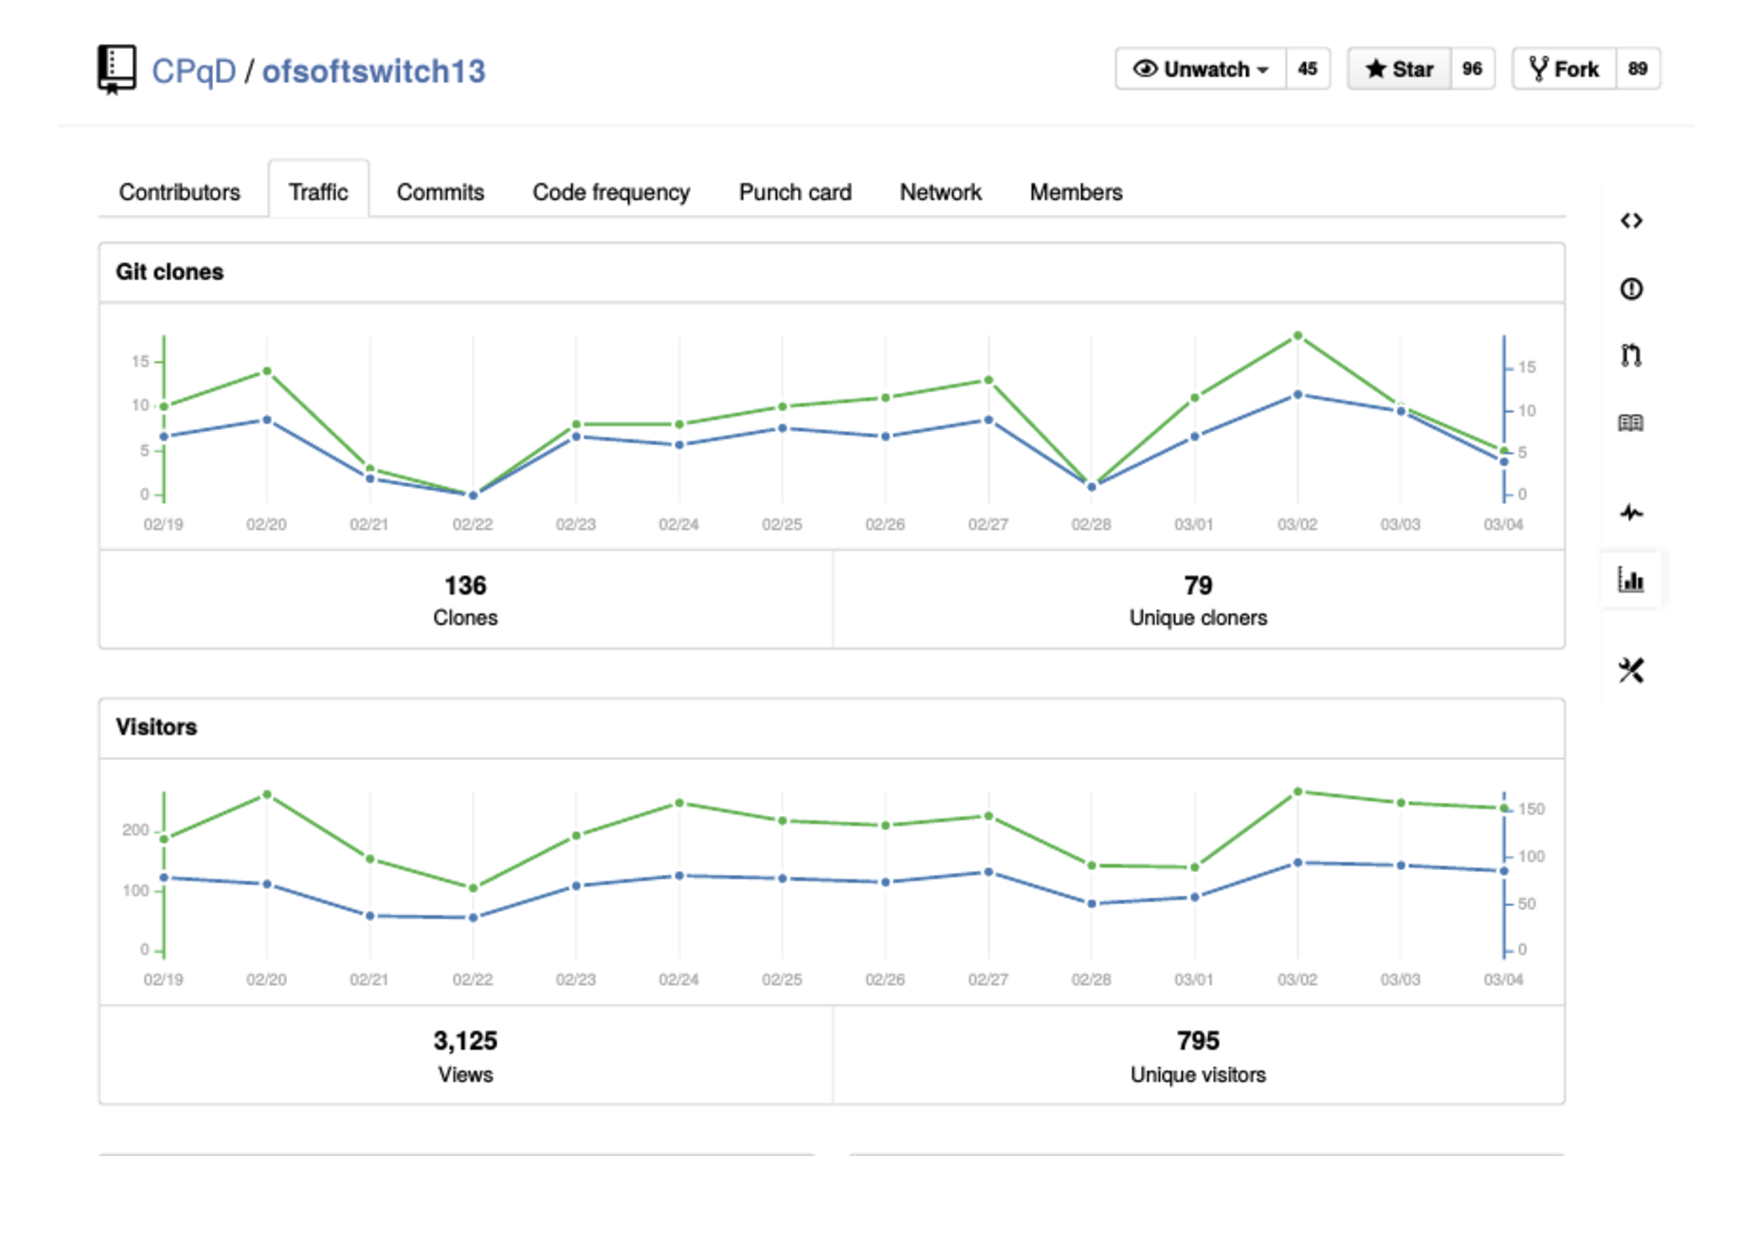
\includegraphics[height=20cm,width=\textwidth,keepaspectratio]{cap5/GH.pdf}
\caption{GitHub statistics.}
\label{fig:ghstats}
\end{figure}

\item \textbf{Part of Mininet installation options.} The software switch is included among the installation options of Mininet. It makes easier for users to start experimenting with OpenFlow 1.3. In addition, the range of people trying     

\item \textbf{Publications.} This work gave origin to three publications. The first paper is about IPv6 support on OpenFlow. The second is an invited paper bringing perspectives on SDN for home network. These ideas were inspired by the software switch port to OpenWRT. Finally, the last paper is an overall presentation of this project, highlighting architectural and implementation details. These publications are listed on Annex \ref{AnnexB}.  
\end{itemize}


\section{Use Cases}
\label{sec:cases}

Known use cases show that the software is an important tool in the advance of the state of art on SDN research and development. As there is a large number of projects that are using or have made use of our work, we will list some notorious examples: 

\begin{itemize}
\item \textbf{Base for new OpenFlow features implementation.} The ONF group responsible by the addition of new OpenFlow features decided to publish new features only if properly implemented and tested. As OpenFlow 1.3 basic functionalities is required for 1.4, the Extensions Work Group chose our work as one of the base software switches used for new functionality prototyping \cite{ONFproto}. 

\item \textbf{Academic.} The software switch has found good adoption by the academic community. For instance, works published in renowned conferences \cite{Reitblatt:2013:FDF:2491185.2491187} \cite{Bianchi:2014:OPP:2602204.2602211} and master dissertations \cite{Paris} \cite{ShahmirShourmasti656472} cite our software as the OpenFlow 1.3 switch chosen for their experiments .  

\item \textbf{Industry.} Industrial development is harder to track because it is usually closed. However, one successful case is in the development of an application for the Open Network Operating System (ONOS). Built by two companies' teams, Dell and ON.Lab, the Segment Routing implementation used the software switch for its simplicity \cite{ONOS}.         
\end{itemize}

\section{Future Work}

Each architectural component from the software switch has space for improvements. New algorithms and data structures are objects of study for the Flow Table matching. More complex and precise algorithms for rate limiting might be considered for Meter Table better performance. As for groups, new bucket select types may be a subject for academic research. 

While there are open ideas for further research and development, some optimizations and features are planned for the software switch in the medium-term. These major improvements are listed below:

\begin{itemize}

\item \textbf{Support for OpenFlow 1.4}. OpenFlow 1.4 is an expansion of OpenFlow 1.3 and it would good to keep the pace with the OpenFlow evolution. Some OpenFlow 1.4 features are already implemented, as stated in section \ref{sec:cases}. However, we would like to have both versions supported in a single switch running instance, without need to split the code in two different programs.

\item \textbf{Hash based match.} Results found in experiments presented on section \ref{sec:bandflows} show a huge loss in performance due to linear matching. To solve this problem, flows entries might be represented as hash value into the Flow Table. Then, packet fields could also be turned into a hash and looked up in the Flow Table. This would give constant performance for the Flow Table look up. However, some relevant questions arise: 

    \begin{itemize}
    \item How to handle flow priority? Since flows should be matched in order of priority, how to ensure the first hash value for a flow is the one with higher priority? 
    \item How to deal with field masking? Some flow match fields may have a mask, so they should be considered in the hash calculation. The question is how to efficiently search and apply these masks to the packet hash calculation. 
    \end{itemize}

The search for an answer for these questions opens space for new research in OpenFlow and SDN, since these questions are not only related to the software switch. 
  
\item \textbf{New packet parsing engine}. The software switch relies on Netbee library to parse packets. While Netbee adds flexibility and extensibility for the parsing and ease the addition of new protocols to OpenFlow, its code is not frequently updated, not following dependencies upgrades. This breaks the software switch compilation in more recent Linux versions, because of more recent versions of libraries required by Netbee. After   Due to the number of compilation issues related to netbee, a new packet parsing module must replace the current third party library.

\end{itemize}


% --- Finaliza a parte no bookmark do PDF, para que se inicie o bookmark na raiz ---
\bookmarksetup{startatroot}%
% ---


% ---- ELEMENTOS P\'{O}S-TEXTUAIS ----
\postextual

% ---- Refer\^{e}ncias bibliogr\'{a}ficas ----
\bibliography{tese}

% ---- Ap\^{e}ndices ----

% ---
% Inicia os ap\^{e}ndices
% ---
%\begin{apendicesenv}
%
%% Imprime uma p\'{a}gina indicando o in\'{\i}cio dos ap\^{e}ndices
%\partapendices
%
%% ----------------------------------------------------------
%\chapter{Quisque libero justo}
%% ----------------------------------------------------------
%
%\lipsum[50]
%
%% ----------------------------------------------------------
%\chapter{Nullam elementum urna vel imperdiet sodales elit ipsum pharetra ligula
%ac pretium ante justo a nulla curabitur tristique arcu eu metus}
%% ----------------------------------------------------------
%\lipsum[55-57]
%
%\end{apendicesenv}
% ---

% ---- Anexos ----

% ---
% Inicia os anexos - opcional
% ---
\begin{anexosenv}

% Imprime uma p\'{a}gina indicando o in\'{\i}cio dos anexos
\partanexos

\chapter{NetPDL packet description example}
\label{annex:NetPDLdesc}

\begin{lstlisting}[frame=single,language=XML,breaklines=true, tabsize=2,showspaces=false,showstringspaces=false]  % Start your code-block

<protocol name="udp" longname="UDP (User Datagram protocol)"         showsumtemplate="udp">
	<format>
		<fields>
			<field type="fixed" name="sport" longname="{0x8000 15}" size="2" showtemplate="FieldDec"/>
			<field type="fixed" name="dport" longname="{0x8000 16}" size="2" showtemplate="FieldDec"/>
			<field type="fixed" name="len" longname="Payload length" size="2" showtemplate="FieldDec"/>
			<field type="fixed" name="crc" longname="Checksum" size="2" showtemplate="FieldHex"/>
		</fields>
	</format>
	<visualization>
		<showsumtemplate name="udp">
			<section name="next"/>
			<text value="UDP: port "/>
			<protofield name="sport" showdata="showvalue"/>
			<text value=" => "/>
			<protofield name="dport" showdata="showvalue"/>
		</showsumtemplate>
	</visualization>
</protocol>     

\end{lstlisting}

% ---
\chapter{Publications}
% ---
\label{AnnexB}
Three papers were published during this work and are listed below. 

\begin{itemize}

    \item Eder Leão Fernandes, Christian Esteve Rothenberg. "OpenFlow 1.3 Software Switch". In Salão de Ferramentas XXXII Simpósio Brasileiro de Redes de Computadores - SBRC'2014, Florianópolis, 5 a 9 de Maio de 2014.

    \item  E. L. Fernandes, C. Esteve Rothenberg and M. R. Salvador. "Software Defined Home Networking: Research Challenges and Innovation Opportunities."(invited paper), In International Workshop on Telecommunications (IWT'13), Santa Rita do Sapucaí, Brazil, 6-9 May 2013
    
    \item Rodrigo R. Denicol, Eder L. Fernandes, Christian E. Rothenberg, Zoltán Lajos Kis, "On IPv6 support in OpenFlow via Flexible Match Structures". OFELIA/CHANGE Summer School SummerSchool, Poster session, Berlin, Germany, November 7-11 November 2011.
    

\end{itemize}

\chapter{Full Ryu Certification test results }
\label{annex:ryucert}

\begin{minipage}[t][5cm][b]{\textwidth}
\begin{tabular}{|l|l|l|}
\hline
\textbf{Ryu Certification Resume} &  &  \\ \hline
 &  &  \\ \hline
\textbf{ofsoftswitch13} & OK & ERROR \\ \hline
Action & 50 & 6 \\ \hline
(Required) & (3) & (0) \\ \hline
(Optional) & (47) & (6) \\ \hline
set\_field & 159 & 7 \\ \hline
(Optional) & (159) & (7) \\ \hline
Match & 708 & 6 \\ \hline
(Required) & (108) & (0) \\ \hline
(Optional) & (600) & (6) \\ \hline
Group & 15 & 0 \\ \hline
(Required) & (3) & (0) \\ \hline
(Optional) & (12) & (0) \\ \hline
Meter & 30 & 6 \\ \hline
(Optional) & (30) & (6) \\ \hline
Total & 962 & 25 \\ \hline
(Required) & (114) & (0) \\ \hline
(Optional) & (848) & (25) \\ \hline
\end{tabular}
\end{minipage} 

\section{Action Tests}
% Please add the following required packages to your document preamble:
% \usepackage{graphicx}
\begin{table}[H]
\centering
\resizebox{\textwidth}{!}{%
\begin{tabular}{|l|l|l|l|l|}
\hline
\textbf{Action} & Required & IPv4 & IPv6 & ARP \\ \hline
OUTPUT & x & OK & OK & OK \\ \hline
PUSH\_VLAN & - & OK & OK & OK \\ \hline
PUSH\_MPLS & - & OK & OK & OK \\ \hline
PUSH\_PBB & - & OK & OK & OK \\ \hline
PUSH\_VLAN (multiple) & - & ERROR & ERROR & ERROR \\ \hline
POP\_VLAN & - & OK & OK & OK \\ \hline
COPY\_TTL\_OUT & - & OK & OK & {[}{]}(\#069a36adbdd0739563365540be6e9b28) \\ \hline
COPY\_TTL\_IN & - & OK & OK & {[}{]}(\#4f5d77f1fc49b1b854e116048c24058d) \\ \hline
SET\_MPLS\_TTL & - & OK & OK & OK \\ \hline
DEC\_MPLS\_TTL & - & OK & OK & OK \\ \hline
PUSH\_MPLS (multiple) & - & OK & OK & OK \\ \hline
POP\_MPLS & - & OK & OK & OK \\ \hline
PUSH\_PBB (multiple) & - & OK & OK & OK \\ \hline
POP\_PBB & - & ERROR & ERROR & ERROR \\ \hline
\end{tabular}
}
\end{table}

\begin{table}[H]
\begin{tabular}{|l|l|l|l|l|l|}
\hline
\textbf{Decrease TLL} & Required & ether & vlan & mpls & pbb \\ \hline
SET\_NW\_TTL (IPv4)   & -        & OK    & OK   & OK   & OK  \\ \hline
DEC\_NW\_TTL (IPv4)   & -        & OK    & OK   & OK   & OK  \\ \hline
SET\_NW\_TTL (IPv6)   & -        & OK    & OK   & OK   & OK  \\ \hline
DEC\_NW\_TTL (IPv6)   & -        & OK    & OK   & OK   & OK  \\ \hline
\end{tabular}
\end{table}

\begin{table}[H]
\begin{tabular}{|l|l|l|l|l|}
\hline
\textbf{set\_field} & Required & IPv4  & IPv6  & ARP   \\ \hline
ETH\_DST            & -        & OK    & OK    & OK    \\ \hline
ETH\_SRC            & -        & OK    & OK    & OK    \\ \hline
ETH\_TYPE           & -        & OK    & OK    & OK    \\ \hline
TUNNEL\_ID          & -        & OK    & OK    & OK    \\ \hline
VLAN\_VID           & -        & OK    & OK    & OK    \\ \hline
VLAN\_PCP           & -        & OK    & OK    & OK    \\ \hline
MPLS\_LABEL         & -        & OK    & OK    & OK    \\ \hline
MPLS\_TC            & -        & OK    & OK    & OK    \\ \hline
MPLS\_BOS           & -        & OK    & OK    & OK    \\ \hline
PBB\_ISID           & -        & ERROR & ERROR & ERROR \\ \hline
\end{tabular}
\end{table}

\begin{table}[H]
\begin{tabular}{|l|l|l|l|l|l|}
\hline
\textbf{set\_field} & Required & ether & vlan  & mpls  & pbb   \\ \hline
IP\_DSCP (IPv4)     & -        & OK    & OK    & OK    & OK    \\ \hline
IP\_ECN (IPv4)      & -        & OK    & OK    & OK    & OK    \\ \hline
IP\_PROTO (IPv4)    & -        & ERROR & ERROR & ERROR & ERROR \\ \hline
IPV4\_SRC           & -        & OK    & OK    & OK    & OK    \\ \hline
IPV4\_DST           & -        & OK    & OK    & OK    & OK    \\ \hline
TCP\_SRC (IPv4)     & -        & OK    & OK    & OK    & OK    \\ \hline
TCP\_DST (IPv4)     & -        & OK    & OK    & OK    & OK    \\ \hline
UDP\_SRC (IPv4)     & -        & OK    & OK    & OK    & OK    \\ \hline
UDP\_DST (IPv4)     & -        & OK    & OK    & OK    & OK    \\ \hline
SCTP\_SRC (IPv4)    & -        & OK    & OK    & OK    & OK    \\ \hline
SCTP\_DST (IPv4)    & -        & OK    & OK    & OK    & OK    \\ \hline
ICMPV4\_TYPE        & -        & OK    & OK    & OK    & OK    \\ \hline
ICMPV4\_CODE        & -        & OK    & OK    & OK    & OK    \\ \hline
IP\_DSCP (IPv6)     & -        & OK    & OK    & OK    & OK    \\ \hline
IP\_ECN (IPv6)      & -        & OK    & OK    & OK    & OK    \\ \hline
TCP\_SRC (IPv6)     & -        & OK    & OK    & OK    & OK    \\ \hline
TCP\_DST (IPv6)     & -        & OK    & OK    & OK    & OK    \\ \hline
UDP\_SRC (IPv6)     & -        & OK    & OK    & OK    & OK    \\ \hline
UDP\_DST (IPv6)     & -        & OK    & OK    & OK    & OK    \\ \hline
SCTP\_SRC (IPv6)    & -        & OK    & OK    & OK    & OK    \\ \hline
SCTP\_DST (IPv6)    & -        & OK    & OK    & OK    & OK    \\ \hline
IPV6\_SRC           & -        & OK    & OK    & OK    & OK    \\ \hline
IPV6\_DST           & -        & OK    & OK    & OK    & OK    \\ \hline
IPV6\_FLABEL        & -        & OK    & OK    & OK    & OK    \\ \hline
ICMPV6\_TYPE        & -        & OK    & OK    & OK    & OK    \\ \hline
ICMPV6\_CODE        & -        & OK    & OK    & OK    & OK    \\ \hline
IPV6\_ND\_TARGET    & -        & OK    & OK    & OK    & OK    \\ \hline
IPV6\_ND\_SLL       & -        & OK    & OK    & OK    & OK    \\ \hline
IPV6\_ND\_TLL       & -        & OK    & OK    & OK    & OK    \\ \hline
ARP\_OP             & -        & OK    & OK    & OK    & OK    \\ \hline
ARP\_SPA            & -        & OK    & OK    & OK    & OK    \\ \hline
ARP\_TPA            & -        & OK    & OK    & OK    & OK    \\ \hline
ARP\_SHA            & -        & OK    & OK    & OK    & OK    \\ \hline
ARP\_THA            & -        & OK    & OK    & OK    & OK    \\ \hline
\end{tabular}
\end{table}

\section{Match Tests}

% Please add the following required packages to your document preamble:
% \usepackage{graphicx}
\begin{table}[H]
\centering
\resizebox{\textwidth}{!}{%
\begin{tabular}{|l|l|l|l|l|l|}
\hline
\textbf{Match}     & Req & ether        & vlan      & mpls         & pbb          \\ \hline
IP\_DSCP (IPv4)    & -   & OK/OK /OK    & OK/OK /OK & OK/OK /OK    & OK/OK /OK    \\ \hline
IP\_ECN (IPv4)     & -   & OK/OK /OK    & OK/OK /OK & OK/OK /OK    & OK/OK /OK    \\ \hline
IP\_PROTO (IPv4)   & x   & OK/OK /OK    & OK/OK /OK & OK / OK / OK & OK/OK /OK    \\ \hline
IPV4\_SRC          & x   & OK/OK /OK    & OK/OK /OK & OK/OK /OK    & OK/OK /OK    \\ \hline
IPV4\_SRC (Mask)   & x   & OK/OK /OK    & OK/OK /OK & OK/OK /OK    & OK/OK /OK    \\ \hline
IPV4\_DST          & x   & OK/OK /OK    & OK/OK /OK & OK/OK /OK    & OK/OK /OK    \\ \hline
IPV4\_DST (Mask)   & x   & OK/OK /OK    & OK/OK /OK & OK/OK /OK    & OK/OK /OK    \\ \hline
TCP\_SRC (IPv4)    & x   & OK/OK /OK    & OK/OK /OK & OK/OK /OK    & OK/OK /OK    \\ \hline
TCP\_DST (IPv4)    & x   & OK/OK /OK    & OK/OK /OK & OK/OK /OK    & OK/OK /OK    \\ \hline
UDP\_SRC (IPv4)    & x   & OK/OK /OK    & OK/OK /OK & OK/OK /OK    & OK/OK /OK    \\ \hline
UDP\_DST (IPv4)    & x   & OK/OK /OK    & OK/OK /OK & OK/OK /OK    & OK/OK /OK    \\ \hline
SCTP\_SRC (IPv4)   & -   & OK/OK /OK    & OK/OK /OK & OK/OK /OK    & OK/OK /OK    \\ \hline
SCTP\_DST (IPv4)   & -   & OK / OK / OK & OK/OK /OK & OK/OK /OK    & OK/OK /OK    \\ \hline
ICMPV4\_TYPE       & -   & OK/OK /OK    & OK/OK /OK & OK/OK /OK    & OK/OK /OK    \\ \hline
ICMPV4\_CODE       & -   & OK/OK /OK    & OK/OK /OK & OK/OK /OK    & OK/OK /OK    \\ \hline
IP\_DSCP (IPv6)    & -   & OK/OK /OK    & OK/OK /OK & OK/OK /OK    & OK/OK /OK    \\ \hline
IP\_ECN (IPv6)     & -   & OK/OK /OK    & OK/OK /OK & OK/OK /OK    & OK/OK /OK    \\ \hline
IP\_PROTO (IPv6)   & x   & OK/OK /OK    & OK/OK /OK & OK/OK /OK    & OK/OK /OK    \\ \hline
TCP\_SRC (IPv6)    & x   & OK/OK /OK    & OK/OK /OK & OK/OK /OK    & OK/OK /OK    \\ \hline
TCP\_DST (IPv6)    & x   & OK/OK /OK    & OK/OK /OK & OK/OK /OK    & OK/OK /OK    \\ \hline
UDP\_SRC (IPv6)    & x   & OK/OK /OK    & OK/OK /OK & OK/OK /OK    & OK/OK /OK    \\ \hline
UDP\_DST (IPv6)    & x   & OK/OK /OK    & OK/OK /OK & OK/OK /OK    & OK/OK /OK    \\ \hline
SCTP\_SRC (IPv6)   & -   & OK/OK /OK    & OK/OK /OK & OK/OK /OK    & OK/OK /OK    \\ \hline
SCTP\_DST (IPv6)   & -   & OK/OK /OK    & OK/OK /OK & OK/OK /OK    & OK/OK /OK    \\ \hline
IPV6\_SRC          & x   & OK/OK /OK    & OK/OK /OK & OK/OK /OK    & OK/OK /OK    \\ \hline
IPV6\_SRC (Mask)   & x   & OK/OK /OK    & OK/OK /OK & OK/OK /OK    & OK/OK /OK    \\ \hline
IPV6\_DST          & x   & OK/OK /OK    & OK/OK /OK & OK/OK /OK    & OK/OK /OK    \\ \hline
IPV6\_DST (Mask)   & x   & OK/OK /OK    & OK/OK /OK & OK/OK /OK    & OK/OK /OK    \\ \hline
IPV6\_FLABEL       & -   & OK/OK /OK    & OK/OK /OK & OK/OK /OK    & OK/OK /OK    \\ \hline
IPV6\_FLABEL(Mask) & -   & OK/OK /OK    & OK/OK /OK & OK/OK /OK    & OK/OK /OK    \\ \hline
ICMPV6\_TYPE       & -   & OK/OK /OK    & OK/OK /OK & OK/OK /OK    & OK/OK /OK    \\ \hline
ICMPV6\_CODE       & -   & OK/OK /OK    & OK/OK /OK & OK/OK /OK    & OK/OK /OK    \\ \hline
IPV6\_ND\_TARGET   & -   & OK/OK /OK    & OK/OK /OK & OK/OK /OK    & OK/OK /OK    \\ \hline
IPV6\_ND\_SLL      & -   & OK/OK /OK    & OK/OK /OK & OK/OK /OK    & OK/OK /OK    \\ \hline
IPV6\_ND\_TLL      & -   & OK/OK /OK    & OK/OK /OK & OK/OK /OK    & OK/OK /OK    \\ \hline
IPV6\_EXTHDR       & -   & OK/OK /OK    & OK/OK /OK & OK/OK /OK    & OK/OK /OK    \\ \hline
IPV6\_EXTHDR(Mask) & -   & OK/OK /OK    & OK/OK /OK & OK/OK 
/OK    & OK/OK /OK    \\ \hline
\end{tabular}
}
\end{table}

\begin{table}[H]
\centering
\resizebox{\textwidth}{!}{%
\begin{tabular}{|l|l|l|l|l|l|}
\hline
\textbf{Match}     & Req & ether        & vlan      & mpls         & pbb          \\ \hline
ARP\_OP            & -   & OK/OK /OK    & OK/OK /OK & OK/OK /OK    & OK/OK /OK    \\ \hline
ARP\_SPA           & -   & OK/OK /OK    & OK/OK /OK & OK/OK /OK    & OK/OK /OK    \\ \hline
ARP\_SPA (Mask)    & -   & OK/OK /OK    & OK/OK /OK & OK/OK /OK    & OK/OK /OK    \\ \hline
ARP\_TPA           & -   & OK/OK /OK    & OK/OK /OK & OK/OK /OK    & OK/OK /OK    \\ \hline
ARP\_TPA (Mask)    & -   & OK/OK /OK    & OK/OK /OK & OK/OK /OK    & OK/OK /OK    \\ \hline
ARP\_SHA           & -   & OK/OK /OK    & OK/OK /OK & OK/OK /OK    & OK / OK / OK \\ \hline
ARP\_SHA (Mask)    & -   & OK/OK /OK    & OK/OK /OK & OK/OK /OK    & OK/OK /OK    \\ \hline
ARP\_THA           & -   & OK/OK /OK    & OK/OK /OK & OK/OK /OK    & OK/OK /OK    \\ \hline
ARP\_THA (Mask)    & -   & OK/OK /OK    & OK/OK /OK & OK/OK /OK    & OK/OK /OK    \\ \hline
\end{tabular}
}
\end{table}

% Please add the following required packages to your document preamble:
% \usepackage{graphicx}
\begin{table}[H]
\centering
\resizebox{\textwidth}{!}{%
\begin{tabular}{|l|l|l|l|l|}
\hline
\textbf{Match} & Required & IPv4 & IPv6 & ARP \\ \hline
IN\_PORT & x & OK / OK / OK & OK / OK / OK & OK / OK / OK \\ \hline
METADATA & - & OK / OK / OK & OK / OK / OK & OK / OK / OK \\ \hline
METADATA (Mask) & - & OK / OK / OK & OK / OK / OK & OK / OK / OK \\ \hline
ETH\_DST & x & OK / OK / OK & OK / OK / OK & OK / OK / OK \\ \hline
ETH\_DST (Mask) & x & OK / OK / OK & OK / OK / OK & OK / OK / OK \\ \hline
ETH\_SRC & x & OK / OK / OK & OK / OK / OK & OK / OK / OK \\ \hline
ETH\_SRC (Mask) & x & OK / OK / OK & OK / OK / OK & OK / OK / OK \\ \hline
ETH\_TYPE & x & OK / OK / OK & OK / OK / OK & OK / OK / OK \\ \hline
TUNNEL\_ID & - & OK / OK / OK & OK / OK / OK & OK / OK / OK \\ \hline
TUNNEL\_ID (Mask) & - & OK / OK / OK & OK / OK / OK & OK / OK / OK \\ \hline
VLAN\_VID & - & OK / OK / OK & OK / OK / OK & OK / OK / OK \\ \hline
VLAN\_VID (Mask) & - & OK / OK / OK & OK / OK / OK & OK / OK / OK \\ \hline
VLAN\_PCP & - & OK / OK / OK & OK / OK / OK & OK / OK / OK \\ \hline
MPLS\_LABEL & - & OK / OK / OK & OK / OK / OK & OK / OK / OK \\ \hline
MPLS\_TC & - & OK / OK / OK & OK / OK / OK & OK / OK / OK \\ \hline
MPLS\_BOS & - & OK / OK / OK & OK / OK / OK & OK / OK / OK \\ \hline
PBB\_ISID & - & ERROR / OK / OK & ERROR / OK / OK & ERROR / OK / OK \\ \hline
PBB\_ISID (Mask) & - & ERROR / OK / OK & ERROR / OK / OK & ERROR / OK / OK \\ \hline
\end{tabular}
}
\end{table}

\section{Group Tests}

\begin{table}[H]
\begin{tabular}{|l|l|l|l|l|}
\hline
\textbf{Group}        & Required & IPv4 & IPv6 & ARP \\ \hline
ALL                   & x        & OK   & OK   & OK  \\ \hline
SELECT\_Ether         & -        & OK   & OK   & OK  \\ \hline
SELECT\_IP            & -        & OK   & OK   & OK  \\ \hline
SELECT\_Weight\_Ether & -        & OK   & OK   & OK  \\ \hline
SELECT\_Weight\_IP    & -        & OK   & OK   & OK  \\ \hline
\end{tabular}
\end{table}

\section{Meter Tests}

\begin{table}[H]
\begin{tabular}{|l|l|l|l|l|}
\hline
\textbf{Meter}                     & Required & IPv4  & IPv6  & ARP   \\ \hline
DROP\_00\_KBPS\_00\_1M             & -        & OK    & OK    & OK    \\ \hline
DROP\_00\_KBPS\_01\_10M            & -        & OK    & OK    & OK    \\ \hline
DROP\_00\_KBPS\_02\_100M           & -        & OK    & OK    & OK    \\ \hline
DROP\_01\_PKTPS\_00\_100           & -        & OK    & OK    & OK    \\ \hline
DROP\_01\_PKTPS\_01\_1000          & -        & OK    & OK    & OK    \\ \hline
DROP\_01\_PKTPS\_02\_10000         & -        & OK    & OK    & OK    \\ \hline
DSCP\_REMARK\_00\_KBPS\_00\_1M     & -        & OK    & OK    & OK    \\ \hline
DSCP\_REMARK\_00\_KBPS\_01\_10M    & -        & OK    & OK    & OK    \\ \hline
DSCP\_REMARK\_00\_KBPS\_02\_100M   & -        & ERROR & ERROR & ERROR \\ \hline
DSCP\_REMARK\_01\_PKTPS\_00\_100   & -        & OK    & OK    & OK    \\ \hline
DSCP\_REMARK\_01\_PKTPS\_01\_1000  & -        & OK    & OK    & OK    \\ \hline
DSCP\_REMARK\_01\_PKTPS\_02\_10000 & -        & ERROR & ERROR & ERROR \\ \hline
\end{tabular}
\end{table}

\label{annex:NetPDLdesc}

\end{anexosenv}

% ---- INDICE REMISSIVO ----

\printindex

\end{document} 
